% XeLaTeX 由 HITSZ build 脚本调用，避免 program 注释绕过多遍编译配方。
% !LW recipe = HITSZ build
% 硕士学位论文工作稿；版式对齐深圳校区学术型硕士官方 LaTeX 范例（hithesisbook）。
\documentclass[fontset=fandol,type=master,campus=harbin,chapterbold=false,tocblank=false]{hithesisbook}
% !TeX root = ../main.tex
% 类文件已提供数学、图表、双语题注和引用支持。
\usepackage{bm}
\usepackage{url}
\usepackage{mathrsfs}
\usepackage{pifont}
\newcommand{\optstar}{\text{\ding{75}}}

% !TeX root = ../main.tex
% 西文 TeX Gyre Termes X / Heros / Cursor 与数学 newtxmath 已由 hithesisbook 类统一启用；
% 此处仅保留求和符号兼容补丁。
\DeclareSymbolFont{LMlargesymbols}{OMX}{lmex}{m}{n}
\DeclareMathSymbol{\LMsum}{\mathop}{LMlargesymbols}{"50}
\renewcommand{\sum}{\LMsum}

% !TeX root = ../main.tex
% 保留中期 algorithm2e 样式；算法配置集中在此，不修改学校类文件。
\usepackage{needspace}
\usepackage[linesnumbered,ruled,lined]{algorithm2e}
\renewcommand{\algorithmcfname}{算法}
\counterwithin{algocf}{chapter}
\renewcommand{\thealgocf}{\thechapter-\arabic{algocf}}
% 输入、输出中文；正文和标题使用模板规定的五号字。
\SetKwInput{KwIn}{输入}
\SetKwInput{KwOut}{输出}
\SetAlFnt{\wuhao}
\SetAlCapFnt{\wuhao}
\SetAlCapNameFnt{\wuhao}
\SetAlCapSty{textnormal}
\SetAlCapNameSty{textnormal}
\SetAlgoCaptionSeparator{\enspace}
\SetAlCapHSkip{0.5\algomargin}
\setlength{\interspacetitleruled}{3pt}
% 保留竖向块线与 end；行号无冒号，语句末不显示分号。
\SetNlSty{textnormal}{}{}
\SetKwFor{For}{for}{do}{end}
\SetKwIF{If}{ElseIf}{Else}{if}{then}{else if}{else}{end}
\DontPrintSemicolon
% 统一定理类环境编号为“章-序”连字符格式，与图表、公式及算法编号保持一致。
\renewcommand{\theassumption}{\thechapter-\arabic{assumption}}
\renewcommand{\thedefinition}{\thechapter-\arabic{definition}}
\renewcommand{\theproposition}{\thechapter-\arabic{proposition}}
\renewcommand{\thelemma}{\thechapter-\arabic{lemma}}
\renewcommand{\thetheorem}{\thechapter-\arabic{theorem}}
\renewcommand{\thecorollary}{\thechapter-\arabic{corollary}}
\renewcommand{\theremark}{\thechapter-\arabic{remark}}

% !TeX root = ../main.tex
% 仅对本论文的参考文献启用孤行保护，不修改学校类文件。
\makeatletter
% 在环境初始化之后设置，避免被类文件内部的零惩罚值覆盖。
\apptocmd{\thebibliography}{%
  \clubpenalty=10000
  \@clubpenalty=10000
  \widowpenalty=10000
  \interlinepenalty=0
  % 只收紧条目间的附加空隙，保留模板字号和行距。
  \addtolength{\itemsep}{-2pt}
}{}{\PackageError{report-layout}{Bibliography layout patch failed}{}}
\makeatother

\bibliographystyle{hithesis}
\graphicspath{{figs/}{figs/completed_work/}}
\begin{document}
\frontmatter
% !TeX root = ../main.tex
% 中文身份信息和题目来自中期报告；学术型理学硕士及导师职称由用户确认；主副标题按学校规范中文用破折号、英文用冒号。
% 原中期报告日期：2026 年 9 月 15 日，不视为毕业论文提交或答辩日期。
\hitsetup{
  statesecrets={公开},
  natclassifiedindex={O1},
  intclassifiedindex={51},
  ctitlecover={联合优化下的非线性滤波\protect\\——神经网络与输运方法},
  ctitle={联合优化下的非线性滤波——神经网络与输运方法},
  cxueke={理学},
  cstudenttype={学术学位论文},
  csubject={数学},
  caffil={哈尔滨工业大学（深圳）},
  cauthor={张守信},
  csupervisor={严质彬 教授},
  cstudentid={24S058012},
  firstpagecdate={2027年1月},
  cdate={2027年1月},
  etitle={Nonlinear Filtering through Joint Optimization: Neural Networks and Transport Methods},
  exueke={Science},
  esubject={Mathematics},
  eaffil={Harbin Institute of Technology, Shenzhen},
  eauthor={Zhang Shouxin},
  esupervisor={Prof. Yan Zhibin},
  edate={January, 2027},
  ckeywords={非线性滤波,粒子滤波,最优输运,流形降维,条件输运映射},
  ekeywords={nonlinear filtering, particle filtering, optimal transport, manifold dimensionality reduction, conditional transport map}
}
% !TeX root = ../main.tex
\begin{cabstract}
粒子滤波是一种使用经验测度来拟合后验测度的方法，由于其无需正态分布假设，因而广泛适用于非线性系统的状态估计。然而，在实际应用中，传统粒子滤波存在一些固有局限：弱过程噪声乃至零过程噪声系统下，重采样步骤会造成单点塌缩；高维观测场景下，似然权重会集中于个别样本，也就是粒子贫化。

本文引入最优输运与神经网络方法来解决上述局限。在重采样步骤，使用输运变换来代替随机重采样，是解决退化问题的经典方法，但本文额外研究了误差的正交分解理论，具有可解释性。对于高维观测场景，本文在经典的条件输运对抗学习方法基础上，构建了摊销条件输运粒子滤波算法，进而同时提升了精度和在线速度。实验选取了三类问题：一维非线性方程、一维零过程噪声混沌系统及含噪手写数字逐窗识别。实验表明，输运方法为粒子滤波增强了稳健性，而离线摊销大幅减少了神经网络的在线推理开销。
\end{cabstract}
\begin{eabstract}
Particle filtering uses an empirical measure to fit the posterior measure; since it requires no normality assumption, it applies broadly to state estimation in nonlinear systems. In practice, however, traditional particle filters have inherent limitations: under weak or even zero process noise, the resampling step causes particles to collapse to a single point; in high-dimensional observation settings, likelihood weights concentrate on just a few samples, i.e., particle impoverishment.

This paper introduces optimal transport and neural network methods to address these limitations. Replacing random resampling with a transport transformation is a classic approach to handling degeneracy, but here we additionally develop an orthogonal error decomposition theory for clear interpretability. For high-dimensional observations, building on classical conditional transport adversarial learning, we construct an amortized conditional transport particle filter that improves both accuracy and online speed. Experiments cover three problems: a one-dimensional nonlinear equation, a one-dimensional chaotic system with zero process noise, and window-by-window recognition of noisy handwritten digits. The results show that transport methods improve the robustness of particle filtering, while offline amortization substantially reduces the online inference overhead of the neural network.
\end{eabstract}


\makecover
\tableofcontents
\mainmatter
% !TeX root = ../main.tex
%%%%%%%%%%%%%%%%%%%%%%%%%%   1   %%%%%%%%%%%%%%%%%%%%%%%%%%%%%%
\chapter{绪论}[Introduction]

\section{课题背景与意义}

从含噪序贯观测数据递推估计动态系统的隐状态，是导航制导、目标跟踪、地球物理资料同化与视觉感知等领域的基础问题\cite{kalman1960new,bar2001estimation,sarkka2013bayesian}。对于线性正态系统，Kalman 滤波给出了最优递推估计\cite{kalman1960new}。推广到非线性系统时，扩展 Kalman 滤波（EKF）与无迹 Kalman 滤波（UKF）\cite{julier1997new}使用局部近似状态低阶矩的方法，计算简便，在弱非线性场合下效果良好；然而，一旦系统为强非线性或多峰后验，就会产生较大误差。自举粒子滤波（BPF）\cite{gordon1993novel}利用加权经验测度来逼近完整的后验分布。由于不再依赖线性与正态分布假设，粒子滤波方法被广泛用于一般非线性系统的状态估计。

然而，传统粒子滤波在几类场合下存在严重问题。当过程噪声为零时，预测步缺乏随机扩散，重采样只能在已有粒子中筛选和复制，因而会导致粒子退化。而当状态或观测的维数较高时，似然权重的方差会随维数急剧增大\cite{bengtsson2008curse,snyder2008obstacles}，权重会迅速集中到个别粒子，亦即粒子贫化。为了克服上述困难，一个重要的方向是引入最优输运理论\cite{villani2009optimal,reich2013nonparametric}，用确定性变换来替代随机重采样。而面对高维观测，则可以结合低维流形表示与条件输运映射来提高弱噪高维场景下的滤波精度和在线速度。因此，我们的研究为滤波领域提供了丰富的理论解释，并增强了已有滤波算法的稳健性，提升了其速度。

\section{国内外研究现状及分析}

1993 年，Gordon、Salmond 和 Smith 提出自举（Bootstrap）粒子滤波，在不依赖线性化或正态假设的条件下实现了递推 Bayes 状态估计\cite{gordon1993novel}。1994 年，Kong、Liu 和 Wong 围绕序贯重要性采样讨论了权重退化与有效粒子数问题\cite{kong1994sequential}；1996 年，Kitagawa 在重采样中引入分层采样\cite{kitagawa1996monte}。此后，Isard 和 Blake 将粒子滤波用于视觉轮廓实时跟踪\cite{isard1998condensation}，Liu 和 Chen 系统归纳了序贯 Monte Carlo 与重要性重采样通用框架\cite{liu1998sequential}。为改善提议分布，Pitt 和 Shephard 提出辅助粒子滤波（APF）对粒子作观测预筛选\cite{pitt1999filtering}，van der Merwe 等结合无迹变换构造重要性分布提出无迹粒子滤波（UPF）\cite{van2000unscented}，Doucet 等主编的文集\cite{doucet2001sequential}进一步总结了利用条件解析结构降维的 Rao-Blackwellized 粒子滤波（RBPF），该分解思想随后亦成功用于同步定位与建图（SLAM）等问题\cite{montemerlo2002fastslam}。

针对重采样后的粒子贫化，一类工作引入 Markov 链 Monte Carlo（MCMC）移动步骤，如 Gilks 和 Berzuini 的重采样-移动算法\cite{gilks2001following}与 Doucet 等的区块采样方法\cite{doucet2006efficient}，但在线计算开销较高\cite{li2017particle}；另一类工作利用核密度平滑恢复连续采样，如正则化粒子滤波（RPF）\cite{musso2001improving}与核均值漂移粒子滤波（KPF）\cite{chang2005kernel}，但核带宽选择对维数敏感，主要适用于低维连续状态空间。粒子滤波的退化机理与改进策略亦可参见相关综述\cite{li2015particlezh,vanleeuwen2019review}。

最优输运理论提供了避免随机复制的确定性样本变换方法\cite{villani2009optimal,peyre2019computational,ma2019optimaltransportzh}。2012 年，El Moselhy 和 Marzouk 构造了从先验到后验的确定性最优映射\cite{el2012bayesian}；2013 年，Reich 提出集合输运粒子滤波（ETPF）\cite{reich2013nonparametric}，以离散最优耦合的条件重心替代随机重采样，克服了集合 Kalman 滤波\cite{evensen2003ensemble}在非正态后验下的线性近似偏差（渐近偏差）。结合 Cuturi 的熵正则化 Sinkhorn 算法\cite{cuturi2013sinkhorn}，Corenflos 等提出基于熵正则输运的可微粒子滤波（DPF）\cite{corenflos2021differentiable}，缓解了重采样不可微问题。Al-Jarrah 等进一步将后验更新归结为条件最优输运问题，利用神经网络通过极大极小对抗优化学习无需似然权重的条件映射（OTPF）及其摊销形式\cite{aljarrah2023otpf,aljarrah2024brenier,aljarrah2025aotf}。

在神经网络状态空间建模与潜空间滤波方面，Krishnan 等提出深度 Kalman 滤波（DKF）与结构化推断网络\cite{krishnan2015deep,krishnan2017structured}，Gu 等利用循环网络自适应学习提议分布\cite{gu2015neural}，Karl 等的深度变分 Bayes 滤波（DVBF）\cite{karl2016deep}与 Hafner 等的潜动力学模型\cite{hafner2019learning}从高维像素观测中提取紧凑的无记忆潜状态。Revach 等提出以网络学习增益的 KalmanNet\cite{revach2022kalmannet}，而 Greenberg 等指出经超参数调优的经典 Kalman 滤波（OKF）在多组基准上仍具竞争力\cite{greenberg2023optimization}。近期工作进一步探索了基于大语言模型上下文泛化的 LLM-Filter\cite{liu2025onefilterall}、结合潜空间动力学与集合评分滤波的 LD-EnSF\cite{xiao2026ldensf}以及高维表示空间中的局部预测学习\cite{stockl2024localprediction}。

综合现有研究可以看出，离散集合输运（ETPF）虽然消除了多项重采样的随机复制噪声，但它仍依赖似然权重，且新粒子受限于预测粒子的凸包，难以直接推广到高维观测场合。另一方面，神经网络条件输运映射避开了权重计算，但逐步在线对抗训练耗时较长，多步映射的复合也容易累积误差。此外，面对高维观测，这类方法还需要与低维表示学习有效衔接。因此，有必要从统一的视角出发，深入分析离散耦合的误差机理，并进一步探索高维观测下的流形压缩与低开销条件输运滤波。

\section{本文的主要研究内容}

围绕传统粒子滤波在弱过程噪声下的样本塌缩与高维观测下的权重失效问题，本文结合最优输运理论与神经网络流形学习，从离散耦合变换与连续条件映射两个层次研究无复制的后验粒子更新方法。在低维状态空间中，通过求解预测经验分布与加权后验分布之间的最优耦合（及其熵正则近似），以确定性重心变换直接将预测粒子更新为近似后验粒子；在高维观测空间中，利用压缩与还原流形拟合提取低维潜空间表示，并结合无需计算似然权重的条件输运映射对抗学习与静态后验一步累积性质，形成离线统一训练、在线单次前向推理的潜空间摊销条件输运粒子滤波算法，进而在多组低维与高维数值实验中检验了上述方法的有效性。全文各章的具体内容安排如下：
\begin{enumerate}[label=(\arabic*),leftmargin=0pt,labelindent=2\ccwd,itemindent=*,labelsep=0.4em,nosep]
  \item 第1章为绪论，阐述非线性状态估计的课题背景与研究意义，梳理粒子滤波退化改进策略、最优输运滤波方法以及神经网络潜空间滤波的国内外研究现状，并在此基础上分析现有方法的局限性，引出本文的研究脉络。
  \item 第2章介绍本文所需的理论基础（相关严格证明归入文末附录），包括统一的测度推前与核复合记号、递推 Bayes 滤波框架、粒子经验测度近似与重采样表示，进而阐述离散 Kantorovich 耦合与熵正则 Sinkhorn 重采样、经验模内积下的压缩与还原流形拟合理论，以及条件输运映射的极大极小对偶表述、局部序贯观测最优识别准则与静止潜状态下后验分布的一步累积表示性质。
  \item 第3章展开具体算法设计与机理分析，给出自举粒子滤波与集合输运粒子滤波的递推流程，建立完备内积空间上均方误差的四项正交分解，并从理论上证明零过程噪声与确定性演化下传统重采样走向单点塌缩的指数退化规律；随后给出潜空间摊销条件输运粒子滤波算法，并从新粒子取值范围、跨步误差传播、还原偏差与在线计算复杂度四个方面对比四类潜空间更新机制。
  \item 第4章开展数值仿真与对比实验，依次在一维强过程噪声非线性基准、一维零过程噪声混沌 Logistic 模型以及高维含噪 MNIST 手写数字逐窗口序贯识别任务上，将离散集合输运及潜空间摊销条件输运滤波与扩展 Kalman 滤波、集合 Kalman 滤波、自举粒子滤波及逐步在线对抗输运基线进行定量比较，从估计精度、样本多样性与在线推理耗时等方面验证本文理论分析与所提算法的性能表现；最后在结论部分总结全文工作，并讨论研究局限与后续方向。
\end{enumerate}

% !TeX root = ../main.tex
\chapter{非线性滤波与最优输运基础}[Foundations of Nonlinear Filtering and Optimal Transport]
% !TeX root = ../../main.tex
\section{符号定义与说明}\label{cw:app:notation}

\textbf{取值空间与密度导数：}随机变量 $X,Y$ 的取值空间分别记为 $\mathcal S_X,\mathcal S_Y$（上下文讨论单一空间且无歧义时简记为 $\mathcal S$），其上可测集合族记为 $\mathcal B(\mathcal S)$。有限维实向量空间上以体积测度为默认参考测度（状态空间上的体积测度记为 $v_X$），密度导数记为 $p_X(x)=\frac{\mathrm d\mathbb P_X}{\mathrm dv_X}(x)$，条件密度简写时记为 $p(x\mid y)=p_{X\mid Y}(x\mid y)$；一般测度间的密度导数记作 $\frac{\mathrm d\mu}{\mathrm d\nu}$，绝对连续记作 $\mu\ll\nu$。数学期望与概率带分布下标写作 $\mathbb E_{X\sim\mathbb P_X}[\cdot]$ 与 $\mathbb P_X(\cdot)$。

\textbf{概率单纯形与全一向量：}对正整数 $n$，$\mathbb R_+=[0,\infty)$，定义
\begin{equation*}
\Delta^{n-1}:=\left\{\bm w\in\mathbb R_+^n:\sum_{i=1}^n w_i=1\right\},\qquad
\mathbf1_n:=(1,\dots,1)^{\mathrm T}.
\end{equation*}
$\Delta^{n-1}$ 是 $n$ 个非负概率权重组成的集合，上标表示其维数；允许零权重，严格正权重另行说明。

\textbf{单点质量测度与示性函数：}对 $x\in\mathcal S$ 和可测集合 $A\in\mathcal B(\mathcal S)$，
\begin{equation*}
\delta_x(A):=\mathbb I_A(x)=
\begin{cases}1,&x\in A,\\0,&x\notin A,\end{cases}
\qquad \int_{\mathcal S}f(s)\,\mathrm d\delta_x(s)=f(x).
\end{equation*}
$\delta_x$ 是集中于单点 $x$ 的概率测度，与表示概率单纯形的大写 $\Delta$ 不同。

\textbf{概率测度与经验测度：}$\mathcal M(\mathcal S)$ 表示 $\mathcal S$ 上的全体非负测度，概率测度全体记为 $\mathcal M^1(\mathcal S):=\{\mu\in\mathcal M(\mathcal S):\mu(\mathcal S)=1\}$，不得将两者混用。记单点质量测度行数组 $\delta_{x_{1..N}}:=(\delta_{x_1},\dots,\delta_{x_N})$，对权重列向量 $\bm w\in\Delta^{N-1}$，加权与等权经验测度分别记为
\begin{equation*}
\delta_{x_{1..N}}\bm w:=\sum_{i=1}^Nw_i\delta_{x_i},\qquad
\hat{\mathbb P}_{N,\bm w;X}:=\delta_{x_{1..N}}\bm w,\qquad
\hat{\mathbb P}_{N;X}:=\frac1N\delta_{x_{1..N}}\mathbf1_N=\frac1N\sum_{i=1}^N\delta_{x_i}.
\end{equation*}
这里 $x_i$ 是样本实现值，行数组右乘列向量表示测度的有限凸组合。

\textbf{索引排列与滤波阶段：}用 $..$ 表示行排列数组 $x_{1..N}:=(x_1,\dots,x_N)$，用 $:$ 表示列拼接序列 $y_{1:k}:=(y_1,\dots,y_k)^{\mathrm T}$。对样本随机列向量 $X_i\in\mathbb R^{d\times1}$，记
\begin{equation*}
X_{1..N}:=(X_1,\dots,X_N)\in\mathbb R^{d\times N},\qquad
\mathbb P_{X_{1..N}}\text{ 为该样本族的联合分布}.
\end{equation*}
一般二元随机变量的联合分布记为 $\mathbb P_{(X,Y)}$。
上标 $-$ 与 $+$ 分别表示预测与后验阶段。位置变换中的 $X_k$ 表示按列拼接的粒子实现矩阵，每列是一个 $n_x$ 维粒子：
\begin{equation*}
\begin{aligned}
&X_k:=x_k^{(1..N)}:=[x_k^{(1)},\dots,x_k^{(N)}]\in\mathbb R^{n_x\times N},\\
&X_k^\pm:=x_k^{\pm,(1..N)}\in\mathbb R^{n_x\times N}.
\end{aligned}
\end{equation*}
$(\bm T_k)_{ij}$ 表示源粒子 $i$ 对目标粒子 $j$ 的贡献系数，故 $X_k^+=X_k^-\bm T_k$，$\bm T_k=N\bm\Pi_k$。概率分布下标中的 $X_k$ 仍表示状态随机变量，由上下文区分。

\textbf{推前、拉回与对偶配对：}对可测映射 $T:\mathcal S_X\to\mathcal S_Y$，
\begin{equation*}
\begin{aligned}
&(T_*\mu)(B):=\mu(T^{-1}(B)),\qquad T^*f:=f\circ T,\\
&\langle f,\mu\rangle_{\mathcal S}:=\int_{\mathcal S}f(s)\,\mathrm d\mu(s),\qquad
\langle f,T_*\mu\rangle_{\mathcal S_Y}=\langle T^*f,\mu\rangle_{\mathcal S_X}.
\end{aligned}
\end{equation*}
其中 $B\in\mathcal B(\mathcal S_Y)$，函数与测度的对偶配对尖括号须标明测度所在空间，积分对非负可测或相应可积函数使用。$\pi_i$ 表示取第 $i$ 个分量的坐标投影，$\mathbb P_X=X_*\mathbb P$。

\textbf{核复合与测度-核乘积耦合：}对条件转移核 $\kappa:\mathcal S_X\to\mathcal M(\mathcal S_Y)$ 与测度 $\mu\in\mathcal M(\mathcal S_X)$，复合测度记作 $\kappa\circ_m\mu:=\int_{\mathcal S_X}\kappa(x)\,\mu(\mathrm dx)\in\mathcal M(\mathcal S_Y)$；测度-核乘积耦合记作 $\mu\otimes_m\kappa\in\mathcal M(\mathcal S_X\times\mathcal S_Y)$，由此联合分布写作 $\mathbb P_{(X,Y)}=\mathbb P_X\otimes_m\mathbb P_{Y\mid X}$，独立乘积测度 $\mu\otimes\nu$（如 $\mathbb P_X\otimes\mathbb P_Y$）为其特例。

\textbf{联合概率矩阵与条件概率矩阵：}在正质量离散支撑上，记
\begin{equation*}
\begin{aligned}
&a_i:=\mathbb P_X(\{x_i\}),\qquad b_j:=\mathbb P_Y(\{y_j\}),\qquad
\Pi_{ij}:=\mathbb P_{(X,Y)}(\{(x_i,y_j)\}),\\
&P_{Y\mid X;i,j}:=\mathbb P_{Y\mid X=x_i}(\{y_j\})=\Pi_{ij}/a_i,\qquad
P_{X\mid Y;j,i}:=\mathbb P_{X\mid Y=y_j}(\{x_i\})=\Pi_{ij}/b_j.
\end{aligned}
\end{equation*}
条件矩阵的行对应条件变量，列对应被条件化变量；$\bm\Pi=(\Pi_{ij})$ 是联合概率矩阵。$\Pi(\mathbb P_X,\mathbb P_Y)$ 表示具有指定边缘的耦合测度集合，$U(\bm a,\bm b)$ 为其离散矩阵表示，见式~\eqref{cw:eq:coupling-family}、\eqref{cw:eq:transport-polytope}。

\textbf{矩阵与向量运算：}矩阵转置写作 $\bm A^{\mathrm T}$，迹写作 $\operatorname{tr}(\bm A)$，$\operatorname{diag}(\bm u)$ 将向量 $\bm u$ 置于矩阵对角线上；$\odot$、$\oslash$ 分别表示逐元素乘、除，$\otimes_k$ 表示矩阵分块直积。实矩阵迹内积记为 $\langle\bm A\mid\bm B\rangle:=\operatorname{tr}(\bm A^{\mathrm T}\bm B)=\sum_{i,j}A_{ij}B_{ij}$；向量一范数记为 $\|\bm z\|_1:=\sum_i|z_i|$，$\|\bm z\|$ 表示向量二范数。

\textbf{输运代价与熵正则化：}离散代价矩阵记为 $\bm C=(C_{ij})$，其中 $C_{ij}:=c(x_i,y_j)$。相对熵记为 $D_{\mathrm{KL}}(\mu\|\nu):=\int\log(\mathrm d\mu/\mathrm d\nu)\,\mathrm d\mu$（$\mu\ll\nu$ 时），否则为 $+\infty$；$\varepsilon>0$ 为熵正则化参数，$\tau>0$ 为边缘残差容差。

\textbf{平方可积空间与正交投影：}取值于 $\mathbb R^{n_x}$ 的平方可积随机变量空间记为 $\mathcal H:=L^2(\Omega,\mathcal F,\mathbb P;\mathbb R^{n_x})$；闭线性子空间关系记为 $\mathcal W\leqslant\mathcal H$，向 $\mathcal W$ 的正交投影算子与余投影算子分别记为 $\mathscr P_{\mathcal W}$ 与 $\mathscr P_{\mathcal W}^{\perp}$。

\textbf{参数空间、对偶伴随与压缩还原算子：}模型参数随机变量 $\bm\Theta$ 的取值空间记为 $\mathcal S_{\bm\Theta}$，参数实现记为 $\bm\theta\in\mathcal S_{\bm\Theta}$，含参条件密度记为 $p_{Y\mid(Z,\bm\Theta)}(y\mid z,\bm\theta)$。赋范或内积空间上的连续线性对偶与内积伴随算子统一记作上标 ${}^\star$，优化问题的最优解统一记作空心星上标 ${}^{\optstar}$（如 $\bm\theta^{\optstar},\mathscr T_{\Rightarrow}^{\optstar}$），以严格区分伴随运算与最优性。高维观测空间 $\mathcal S_X=\mathbb R^{n_D}$ 与低维潜空间 $\mathcal S_Z=\mathbb R^{n_d}$（$n_d<n_D$）之间的压缩算子与还原算子分别记为 $\mathscr T_{\Rightarrow}:\mathcal S_X\to\mathcal S_Z$ 与 $\mathscr T_{\Leftarrow}:\mathcal S_Z\to\mathcal S_X$，线性情形下二者在标准基下的表示矩阵记为 $\bm T_{\Rightarrow},\bm T_{\Leftarrow}$。


% !TeX root = ../../main.tex
\section{非线性滤波问题}\label{cw:sec:model}

本文从状态空间模型与 Bayes 递推出发，梳理粒子滤波及最优输运重采样的数学关系，并给出算法实现与仿真比较。经典滤波框架与序贯蒙特卡罗方法分别参考文献\cite{bar2001estimation,doucet2001sequential}。

本文约定：凡使用密度公式时，均假设相应密度存在，以相应空间的体积测度为参考测度，密度等式按几乎处处理解。状态空间的体积测度记为 $v_X$。第~\ref{cw:sec:sim-logistic} 节的零过程噪声模型使用单点质量转移核，预测按测度推前理解。

设概率空间为 $(\Omega,\mathcal{F},\mathbb{P})$，状态空间为 $(\mathcal{S}_X,\mathcal{B}(\mathcal{S}_X))$，观测空间为 $(\mathcal{S}_Y,\mathcal{B}(\mathcal{S}_Y))$，其中 $\mathcal{S}_X=\mathbb{R}^{n_x}$，$\mathcal{S}_Y=\mathbb{R}^{n_y}$，$\mathcal{B}$ 表示可测集合族。状态与观测满足
\begin{equation}\label{cw:eq:1}
\begin{aligned}
&X_k=f(X_{k-1},N_{x,k}),\\
&Y_k=h(X_k,N_{y,k}),\;k\geq1.
\end{aligned}
\end{equation}
其中 $X_k:\Omega\to\mathcal{S}_X$，$Y_k:\Omega\to\mathcal{S}_Y$ 为可测映射，$f,h$ 为已知可测函数。$\mathbb{P}$ 定义在 $\Omega$ 上，状态分布 $\mathbb{P}_{X_k}=(X_k)_*\mathbb{P}$ 与滤波后验分布定义在 $\mathcal{S}_X$ 上。

条件：
\begin{itemize}
\item 所有时刻的过程噪声与观测噪声彼此独立，并与 $X_0$ 独立，即 $X_0, N_{x,k}, N_{y,k}$ 作为随机变量相互独立。
\item 观测条件密度 $p_{Y_k\mid X_k}(y \mid x)$ 可计算，对实际观测，Bayes 更新的归一化常数有限且严格为正。
\end{itemize}

输入：模型 $f,h$，初始分布 $\mathbb{P}_{X_0}$，噪声分布 $\mathbb{P}_{N_x},\mathbb{P}_{N_y}$，依次到达的观测值 $y_1,y_2,\dots$。

输出：逐个收到观测 $y_k$，递推求解当前状态的后验概率密度函数 $p_{X_k\mid Y_{1:k}}(x_k \mid y_{1:k})$。

% !TeX root = ../../main.tex
\section{Bayes 滤波}\label{cw:sec:bayes}

\begin{lemma}[无记忆性\cite{sarkka2013bayesian,cappe2005inference}]\label{cw:lem:markov}
在上述状态方程与噪声独立性条件下，给定 $X_{k-1}$ 后，$X_k$ 的条件分布不再依赖更早的状态与历史观测；给定 $X_k$ 后，$Y_k$ 的条件分布不再依赖过去的状态与观测。对 $k\geq1$ 有
\begin{equation}\label{cw:eq:2}
\begin{aligned}
&p_{X_k\mid X_{0:k-1},Y_{1:k-1}}(x_k\mid x_{0:k-1},y_{1:k-1})
=p_{X_k\mid X_{k-1}}(x_k\mid x_{k-1}),\\
&p_{Y_k\mid X_{0:k},Y_{1:k-1}}(y_k\mid x_{0:k},y_{1:k-1})
=p_{Y_k\mid X_k}(y_k\mid x_k).
\end{aligned}
\end{equation}
$k=1$ 时历史观测为空。第一式给出状态的单步无记忆性，第二式给出观测的条件独立性，分别用于下述预测与更新。

\end{lemma}
\begin{proof}
为完整起见，本文给出自行推导的证明：离散情形的证明及一般情形的推广说明见附录~\ref{cw:app:markov-proof}~节。
\end{proof}

固定观测记录 $y_{1:k}=(y_1,\dots,y_k)^{\mathrm{T}}$，以 $p_{X_0}$ 初始化，$k=1$ 时不含历史观测条件。

\textbf{预测：}由上一时刻的后验与状态转移密度，求当前状态在收到 $y_k$ 前的条件密度。
\begin{equation}\label{cw:eq:3}
\begin{aligned}
&p_{X_k\mid Y_{1:k-1}}(x_k\mid y_{1:k-1})\\
= &\int_{\mathcal{S}_X}p_{X_k\mid X_{k-1}}(x_k\mid x_{k-1})p_{X_{k-1}\mid Y_{1:k-1}}(x_{k-1}\mid y_{1:k-1})\,\mathrm{d}v_X(x_{k-1}).
\end{aligned}
\end{equation}

\textbf{更新：}收到 $y_k$ 后，用观测似然对预测密度加权，再归一化，证明见定理~\ref{cw:thm:bayes}。
\begin{equation}\label{cw:eq:4}
\begin{aligned}
&p_{X_k\mid Y_{1:k}}(x_k\mid y_{1:k})\\
= &\frac{p_{Y_k\mid X_k}(y_k\mid x_k)p_{X_k\mid Y_{1:k-1}}(x_k\mid y_{1:k-1})}
{\displaystyle\int_{\mathcal{S}_X}p_{Y_k\mid X_k}(y_k\mid x)p_{X_k\mid Y_{1:k-1}}(x\mid y_{1:k-1})\,\mathrm{d}v_X(x)}.
\end{aligned}
\end{equation}
分母就是观测的预测密度 $p_{Y_k\mid Y_{1:k-1}}(y_k\mid y_{1:k-1})$，要求其有限且严格为正。更新所得后验作为下一步预测的输入，这两步构成精确的 Bayes 滤波递推。

% !TeX root = ../../main.tex
\section{粒子滤波与经验测度近似}\label{cw:sec:particle}

以下以 Gordon 等提出的自举粒子滤波为基础\cite{gordon1993novel}，采用序贯蒙特卡罗的经验测度表示\cite{doucet2001sequential}。粒子滤波的理论框架、主要算法与多目标跟踪应用已有系统的中文综述\cite{li2015particlezh}。

固定观测记录，用 $-$ 与 $+$ 分别表示预测与后验，记
\begin{equation}\label{cw:eq:5}
\begin{aligned}
&\mathbb{P}_{X_k}^-:=\mathbb{P}_{X_k\mid Y_{1:k-1}=y_{1:k-1}},\\
&\mathbb{P}_{X_k}^+:=\mathbb{P}_{X_k\mid Y_{1:k}=y_{1:k}},\\
&\mathbb{P}_{X_0}^+:=\mathbb{P}_{X_0}.
\end{aligned}
\end{equation}

从预测公式出发，以下使用条件密度的简写 $p(x_k\mid y_{1:k-1})=p_{X_k\mid Y_{1:k-1}}(x_k\mid y_{1:k-1})$，其他条件密度同理：
\begin{equation}\label{cw:eq:6}
\begin{aligned}
&p(x_k\mid y_{1:k-1})\\
= &\int_{\mathcal{S}_X}p(x_k\mid x_{k-1})p(x_{k-1}\mid y_{1:k-1})\,\mathrm{d}v_X(x_{k-1}).
\end{aligned}
\end{equation}

固定 $x_k$，这个积分就是函数 $x_{k-1}\mapsto p(x_k\mid x_{k-1})$ 关于上一时刻后验分布的平均。因此，先假设能够从 $p(x_{k-1}\mid y_{1:k-1})$ 独立抽取 $N$ 个样本，记实现值为 $x_{k-1}^{+,(1)},\dots,x_{k-1}^{+,(N)}$，其中 $+$ 表示这些样本来自后验分布。

由简单抽样得到等权经验测度，每个样本占 $1/N$ 的质量：
\begin{equation}\label{cw:eq:7}
\hat{\mathbb{P}}_{N;X_{k-1}}^+
:=\frac1N\sum_{i=1}^N\delta_{x_{k-1}^{+,(i)}}.
\end{equation}
用这一经验测度替换预测积分中的后验测度 $p(x_{k-1}\mid y_{1:k-1})\,\mathrm{d}v_X(x_{k-1})$，得到
\begin{equation}\label{cw:eq:8}
\begin{aligned}
&p(x_k\mid y_{1:k-1})\\
\approx &\int_{\mathcal{S}_X}p(x_k\mid x_{k-1})\,\mathrm{d}\hat{\mathbb{P}}_{N;X_{k-1}}^+(x_{k-1})\\
= &\frac1N\sum_{i=1}^N\int_{\mathcal{S}_X}p(x_k\mid x_{k-1})\,\mathrm{d}\delta_{x_{k-1}^{+,(i)}}(x_{k-1}).
\end{aligned}
\end{equation}
最后使用单点质量测度的积分性质 $\int\varphi(x)\,\mathrm{d}\delta_a(x)=\varphi(a)$，每个积分都变成在对应样本处的函数值：
\begin{equation}\label{cw:eq:9}
p(x_k\mid y_{1:k-1})\approx\frac1N\sum_{i=1}^N p(x_k\mid x_{k-1}^{+,(i)}).
\end{equation}
这样，后验分布下的积分被样本平均近似，预测密度成为 $N$ 个转移密度的等权混合。

\textbf{提议分布：}在生成新粒子时，需要指定实际用于抽样的分布，其密度称为提议密度，记为 $q$。它可以依赖旧粒子与当前观测，抽样操作写作
\begin{equation}\label{cw:eq:10}
x_k^{-,(i)}\sim q(\cdot\mid x_{k-1}^{+,(i)},y_k).
\end{equation}
当前要对上面的预测混合分布进行采样，我们选择每个成分本身的转移密度作为提议密度：
\begin{equation}\label{cw:eq:11}
q(x_k\mid x_{k-1}^{+,(i)},y_k)=p(x_k\mid x_{k-1}^{+,(i)}).
\end{equation}
这一选择在生成粒子时不使用当前观测 $y_k$，正是自举滤波采用的转移先验提议。

\textbf{分层采样：}以混合成分的编号 $i$ 作为分层依据，第 $i$ 层对应密度 $p(x_k\mid x_{k-1}^{+,(i)})$，在混合分布中占 $1/N$ 的质量。因此每层分配一个样本，给定上一时刻的粒子后，各层独立抽取预测粒子：
\begin{equation}\label{cw:eq:12}
x_k^{-,(i)}\sim p(\cdot\mid x_{k-1}^{+,(i)}),\;i=1,\dots,N.
\end{equation}
这里 $\sim$ 表示抽样操作，$x_k^{-,(i)}$ 记抽得的实现值。由状态方程，这一操作可以通过独立抽取过程噪声实现值 $n_{x,k}^{(i)}$ 完成：
\begin{equation}\label{cw:eq:13}
x_k^{-,(i)}=f\bigl(x_{k-1}^{+,(i)},n_{x,k}^{(i)}\bigr).
\end{equation}

在上述转移先验提议下，每个样本代表所在层的 $1/N$ 质量，因此将这些预测粒子合并，得到预测分布的等权经验测度：
\begin{equation}\label{cw:eq:14}
\hat{\mathbb{P}}_{N;X_k}^-:=\frac1N\sum_{i=1}^N\delta_{x_k^{-,(i)}}
\approx\mathbb{P}_{X_k}^-.
\end{equation}
这一步用有限个点质量进一步近似前面得到的混合分布。给定旧粒子后，各层样本独立，但各自服从对应的转移分布。

\textbf{更新：}$-$ 与 $+$ 分别表示使用当前观测前后的预测与后验阶段，此处只更新权重。
对任意可测集合 $A$，将 Bayes 公式中的预测测度替换为等权经验测度，再用单点质量测度的积分性质展开；假设样本似然总和有限且严格为正，约去 $1/N$ 后得到加权后验近似：
\begin{equation}\label{cw:eq:particle-update}
\begin{aligned}
&\mathbb{P}_{X_k}^+(A)\\
={}&\int_A\frac{p(y_k\mid x)p(x\mid y_{1:k-1})}{\displaystyle\int_{\mathcal{S}_X}p(y_k\mid z)p(z\mid y_{1:k-1})\,\mathrm{d}v_X(z)}\,\mathrm{d}v_X(x)\\
={}&\frac{\displaystyle\int_A p(y_k\mid x)\,\mathrm{d}\mathbb{P}_{X_k}^-(x)}{\displaystyle\int_{\mathcal{S}_X}p(y_k\mid x)\,\mathrm{d}\mathbb{P}_{X_k}^-(x)},\\
\Rightarrow\quad &\hat{\mathbb{P}}_{N,\bm w_k^+;X_k}^+(A):=\frac{\displaystyle\int_A p(y_k\mid x)\,\mathrm{d}\hat{\mathbb{P}}_{N;X_k}^-(x)}{\displaystyle\int_{\mathcal{S}_X}p(y_k\mid x)\,\mathrm{d}\hat{\mathbb{P}}_{N;X_k}^-(x)}\\
={}&\sum_{i=1}^N w_k^{+,(i)}\delta_{x_k^{-,(i)}}(A),\\
&w_k^{+,(i)}:=\frac{p(y_k\mid x_k^{-,(i)})}{\displaystyle\sum_{j=1}^N p(y_k\mid x_k^{-,(j)})},\;i=1..N.
\end{aligned}
\end{equation}

\textbf{重采样：}
粗略地说，重采样是对粒子位置的更新。因此，和上一步的概率测度更新应该联为一体，同属于预测 $\to $ 更新的大步骤。
粒子矩阵按列排列为 $X_k^\pm:=x_k^{\pm,(1..N)}\in\mathbb R^{n_x\times N}$。用 $\bm\Pi_k$ 表示联合概率矩阵，$\bm T_k$ 表示位置变换矩阵，$\bm n_k$ 表示各粒子的复制次数，$(\bm T_k)_{ij}$ 表示源粒子 $i$ 对目标粒子 $j$ 的贡献系数。经典重采样中该系数为 $\mathbb I_{\{A_j=i\}}$，其中 $A_j$ 是目标粒子 $j$ 抽取的源索引：
\begin{equation}\label{cw:eq:resampling}
\begin{aligned}
&X_k^+=X_k^-\bm T_k=NX_k^-\bm\Pi_k,\;\bm T_k=N\bm\Pi_k\geq0,\\
&\bm T_k^{\mathrm T}\mathbf1_N=\mathbf1_N,\;\bm T_k\mathbf1_N=\bm n_k,\;\mathbb E[\bm n_k\mid\bm w_k^+]=N\bm w_k^+.
\end{aligned}
\end{equation}
重采样就是按后验权重，从已有预测粒子中有放回地抽取 $N$ 次。先把各粒子的权重依次累加，将 $[0,1)$ 划成 $N$ 段，每段长度就是对应粒子的权重。
每次独立抽一个均匀随机数，落在哪一段，就复制哪一个粒子；重复 $N$ 次，得到后验粒子。因而，权重越大的粒子越容易被多次保留，权重小的粒子可能一次也选不到。
将新粒子的权重统一设为 $1/N$，原来由权重表达的质量差异，就改由复制次数表达。
这样，$\bm T_k$ 的第 $j$ 列记录新粒子 $j$ 复制了谁，$\bm n_k$ 记录每个旧粒子被复制了几次。单次重采样会产生随机误差；固定原粒子与权重后，对重采样随机性取平均，所得经验测度等于原加权测度。

% !TeX root = ../../main.tex
\section{最优输运与重采样}\label{cw:sec:ot}

经典重采样通过随机复制选择耦合矩阵，其源边缘为实际复制比例，只有对重采样随机性取平均后才恢复后验权重：
\begin{equation}\label{cw:eq:ot-random-marginal}
\bm\Pi_k\mathbf1_N=\frac{\bm n_k}{N},\qquad
\bm\Pi_k^{\mathrm T}\mathbf1_N=\frac1N\mathbf1_N,\qquad
\mathbb E_{\bm n_k\sim\mathbb P_{\bm n_k\mid\bm w_k^+}}
\!\left[\frac{\bm n_k}{N}\right]=\bm w_k^+.
\end{equation}
另一种选择是直接约束源边缘为 $\bm w_k^+$，并按粒子间的移动代价选择耦合。为此，先从输运映射出发，建立联合分布、条件概率与离散耦合矩阵之间的关系。

\subsection{从 Monge 映射到 Kantorovich 耦合}\label{cw:sec:monge}

本节采用最优输运的标准映射与耦合表述\cite{villani2009optimal,peyre2019computational}；其基本理论、离散模型与正则化方法亦可参考文献\cite{ma2019optimaltransportzh}。

本节暂用 $X,Y$ 表示一般输运问题的源、目标随机变量，$Y$ 不特指滤波观测。给定边缘分布 $\mathbb P_X,\mathbb P_Y$ 与非负代价函数 $c$，Monge 问题寻找可测映射 $T$，使
\begin{equation}\label{cw:eq:monge}
\begin{aligned}
&Y=T(X),\qquad T_*\mathbb P_X=T_*X_*\mathbb P=\mathbb P_Y,\\
&\inf_{T:\,T_*\mathbb P_X=\mathbb P_Y}
\int_{\mathcal S_X}c(x,T(x))\,\mathrm d\mathbb P_X(x)
=\inf_{T:\,T_*\mathbb P_X=\mathbb P_Y}
\mathbb E_{X\sim\mathbb P_X}[c(X,T(X))].
\end{aligned}
\end{equation}
确定性绑定 $Y=T(X)$ 使条件分布退化为 $\mathbb P_{Y\mid X=x}=\delta_{T(x)}$：一个源点的质量只能整体送往一个目标点，不能拆分。离散边缘因而可能不存在这样的映射；均匀离散分布的整除条件见附录~\ref{cw:app:monge}。

\textbf{耦合松弛：}解除函数绑定，允许任意满足两个边缘约束的联合分布。记坐标投影 $\pi_1(x,y)=x$、$\pi_2(x,y)=y$，定义
\begin{equation}\label{cw:eq:coupling-family}
\Pi(\mathbb P_X,\mathbb P_Y)
:=\left\{\mu\in\mathcal M^1(\mathcal S_X\times\mathcal S_Y):
(\pi_1)_*\mu=\mathbb P_X,\ (\pi_2)_*\mu=\mathbb P_Y\right\}.
\end{equation}
输运目标于是成为联合分布上的期望最小化：
\begin{equation}\label{cw:eq:kantorovich}
\inf_{\mu\in\Pi(\mathbb P_X,\mathbb P_Y)}
\int_{\mathcal S_X\times\mathcal S_Y}c(x,y)\,\mathrm d\mu(x,y)
=\inf_{\mathbb P_{(X,Y)}\in\Pi(\mathbb P_X,\mathbb P_Y)}
\mathbb E_{(X,Y)\sim\mathbb P_{(X,Y)}}[c(X,Y)].
\end{equation}
在有限维实向量空间上，联合分布可通过条件转移核写成测度-核乘积耦合
$\mathbb P_{(X,Y)}=\mathbb P_X\otimes_m\mathbb P_{Y\mid X}$；独立乘积
$\mathbb P_X\otimes\mathbb P_Y$ 是其中一个特例。

\subsection{离散耦合与条件概率及边缘约束}\label{cw:sec:discrete-ot}

设两组支撑点各自互异，$\bm a\in\Delta^{m-1}$、$\bm b\in\Delta^{n-1}$，且暂取 $a_i,b_j>0$；符号定义见第~\ref{cw:app:notation}~节。记
\begin{equation}\label{cw:eq:discrete-coupling}
\begin{aligned}
&\mathbb P_X=\delta_{x_{1..m}}\bm a,\qquad
\mathbb P_Y=\delta_{y_{1..n}}\bm b,\\
&\Pi_{ij}:=\mathbb P_{(X,Y)}(\{(x_i,y_j)\}),\qquad
\mathbb P_{(X,Y)}=\sum_{i=1}^m\sum_{j=1}^n\Pi_{ij}\,
\delta_{x_i}\otimes\delta_{y_j}.
\end{aligned}
\end{equation}
这里 $\otimes$ 表示测度的乘积。对点质量作坐标推前，就得到边缘的行和、列和：
\begin{equation}\label{cw:eq:discrete-marginals}
\begin{aligned}
&(\pi_1)_*(\delta_{x_i}\otimes\delta_{y_j})=\delta_{x_i},\qquad
(\pi_2)_*(\delta_{x_i}\otimes\delta_{y_j})=\delta_{y_j},\\
&(\pi_1)_*\mathbb P_{(X,Y)}=\sum_{i=1}^m\left(\sum_{j=1}^n\Pi_{ij}\right)\delta_{x_i}=\mathbb P_X,\\
&(\pi_2)_*\mathbb P_{(X,Y)}=\sum_{j=1}^n\left(\sum_{i=1}^m\Pi_{ij}\right)\delta_{y_j}=\mathbb P_Y.
\end{aligned}
\end{equation}
函数与测度的对偶配对记为 $\langle f,\mu\rangle_{\mathcal S}:=\int_{\mathcal S}f(s)\,\mathrm d\mu(s)$，下标标明测度所在空间。
对于一般情况（假使需要讨论连续而非离散），等价地，用推前与拉回对偶，对任意可测集合 $A\in\mathcal B(\mathcal S_X)$ 有
\begin{equation}\label{cw:eq:marginal-duality}
\begin{aligned}
\langle\mathbb I_A\otimes\mathbf1_{\mathcal S_Y},\mathbb P_{(X,Y)}\rangle_{\mathcal S_X\times\mathcal S_Y}
&=\langle\pi_1^*\mathbb I_A,\mathbb P_{(X,Y)}\rangle_{\mathcal S_X\times\mathcal S_Y}\\
&=\langle\mathbb I_A,(\pi_1)_*\mathbb P_{(X,Y)}\rangle_{\mathcal S_X}
=\langle\mathbb I_A,\mathbb P_X\rangle_{\mathcal S_X}.
\end{aligned}
\end{equation}
\begingroup\raggedright
更一般地，每个坐标分别满足 $(\pi_i)_*\mathbb P_{X_{1..N}}=\mathbb P_{X_i}$；全部边缘组成的族应写为
$((\pi_i)_*\mathbb P_{X_{1..N}})_{i=1}^N=(\mathbb P_{X_i})_{i=1}^N$。\par
\endgroup

\textbf{条件概率：}条件概率矩阵标明条件方向，联合概率矩阵统一记为 $\bm\Pi$：
\begin{equation}\label{cw:eq:conditional-matrices}
\begin{aligned}
&P_{Y\mid X;i,j}:=\mathbb P_{Y\mid X=x_i}(\{y_j\})=\frac{\Pi_{ij}}{a_i},\qquad
P_{X\mid Y;j,i}:=\mathbb P_{X\mid Y=y_j}(\{x_i\})=\frac{\Pi_{ij}}{b_j},\\
&\bm\Pi=\operatorname{diag}(\bm a)\bm P_{Y\mid X}
=\bm P_{X\mid Y}^{\mathrm T}\operatorname{diag}(\bm b),\\
&\bm P_{Y\mid X}\mathbf1_n=\mathbf1_m,\qquad
\bm P_{Y\mid X}^{\mathrm T}\bm a=\bm b.
\end{aligned}
\end{equation}
条件矩阵以条件变量的取值编号为行、被条件化变量的取值编号为列。

\textbf{离散输运：}令 $C_{ij}=c(x_i,y_j)$，连续耦合约束化为输运多面体，目标化为有限求和：
\begin{equation}\label{cw:eq:transport-polytope}
\begin{aligned}
&U(\bm a,\bm b):=\{\bm\Pi\in\mathbb R_+^{m\times n}:
\bm\Pi\mathbf1_n=\bm a,\ \bm\Pi^{\mathrm T}\mathbf1_m=\bm b\},\\
&\min_{\bm\Pi\in U(\bm a,\bm b)}\langle\bm\Pi\mid\bm C\rangle,
\qquad\langle\bm\Pi\mid\bm C\rangle:=\operatorname{tr}(\bm\Pi^{\mathrm T}\bm C)=\sum_{i=1}^m\sum_{j=1}^n\Pi_{ij}C_{ij}.
\end{aligned}
\end{equation}
独立联合分布对应 $\bm\Pi=\bm a\bm b^{\mathrm T}\in U(\bm a,\bm b)$。

\subsection{熵正则化与 Sinkhorn 迭代}\label{cw:sec:sinkhorn}

采用 Cuturi 的熵正则化离散输运方案\cite{cuturi2013sinkhorn}，推导及数值实现参考文献\cite{peyre2019computational}。

\textbf{正则化：}给定 $\varepsilon>0$，以独立联合分布为参考测度，考虑
\begin{equation}\label{cw:eq:regularized-measure}
\mathbb P_{(X,Y)}^\varepsilon
=\operatorname*{argmin}_{\mu\in\Pi(\mathbb P_X,\mathbb P_Y)}
\left\{\int_{\mathcal S_X\times\mathcal S_Y} c(x,y)\,\mathrm d\mu(x,y)
+\varepsilon D_{\mathrm{KL}}(\mu\|\mathbb P_X\otimes\mathbb P_Y)\right\}.
\end{equation}
在离散边缘固定时，KL 项与负熵仅相差一个常数；以下采用 $0\log0=0$：
\begin{equation}\label{cw:eq:kl-entropy}
\begin{aligned}
D_{\mathrm{KL}}(\bm\Pi\|\bm a\bm b^{\mathrm T})
&=\sum_{i=1}^m\sum_{j=1}^n\Pi_{ij}\log\frac{\Pi_{ij}}{a_i b_j}\\
&=\sum_{i=1}^m\sum_{j=1}^n\Pi_{ij}\log\Pi_{ij}
-\sum_{i=1}^m a_i\log a_i-\sum_{j=1}^n b_j\log b_j.
\end{aligned}
\end{equation}
因此，所求矩阵等价地满足
\begin{equation}\label{cw:eq:regularized-matrix}
\bm\Pi^\varepsilon
=\operatorname*{argmin}_{\bm\Pi\in U(\bm a,\bm b)}
\left\{\langle\bm\Pi\mid\bm C\rangle
+\varepsilon\sum_{i=1}^m\sum_{j=1}^n\Pi_{ij}(\log\Pi_{ij}-1)\right\}.
\end{equation}
这里额外减去 $\varepsilon\sum_{i,j}\Pi_{ij}=\varepsilon$ 也是常数，使求导后的表达更简洁。

\textbf{对偶条件：}取 $\bm\alpha\in\mathbb R^m$、$\bm\beta\in\mathbb R^n$，构造拉格朗日函数：
\begin{equation}\label{cw:eq:sinkhorn-lagrangian}
\begin{aligned}
\mathcal L(\bm\Pi,\bm\alpha,\bm\beta)
={}&\langle\bm\Pi\mid\bm C\rangle
+\varepsilon\sum_{i=1}^m\sum_{j=1}^n\Pi_{ij}(\log\Pi_{ij}-1)\\
&+\bm\alpha^{\mathrm T}(\bm\Pi\mathbf1_n-\bm a)
+\bm\beta^{\mathrm T}(\bm\Pi^{\mathrm T}\mathbf1_m-\bm b).
\end{aligned}
\end{equation}
有限代价与严格正边缘下，最优矩阵各元素严格为正；一阶条件给出
\begin{equation}\label{cw:eq:sinkhorn-scaling}
\begin{aligned}
&\frac{\partial\mathcal L}{\partial\Pi_{ij}}
=C_{ij}+\varepsilon\log\Pi_{ij}+\alpha_i+\beta_j=0,\\
&K_{ij}:=\exp(-C_{ij}/\varepsilon),\qquad
u_i:=\exp(-\alpha_i/\varepsilon),\quad v_j:=\exp(-\beta_j/\varepsilon),\\
&\Pi_{ij}^\varepsilon=u_iK_{ij}v_j,\qquad
\bm\Pi^\varepsilon=\operatorname{diag}(\bm u)\bm K\operatorname{diag}(\bm v).
\end{aligned}
\end{equation}

\textbf{交替缩放：}将矩阵分解代回边缘约束，得到
\begin{equation}\label{cw:eq:sinkhorn-iteration}
\begin{aligned}
&\bm u\odot(\bm K\bm v)=\bm a,\qquad
\bm v\odot(\bm K^{\mathrm T}\bm u)=\bm b,\\
&\bm v^{(0)}=\mathbf1_n,\qquad
\bm u^{(\ell+1)}=\bm a\oslash(\bm K\bm v^{(\ell)}),\\
&\bm v^{(\ell+1)}=\bm b\oslash(\bm K^{\mathrm T}\bm u^{(\ell+1)}),\\
&\bm\Pi^{(\ell+1)}
=\operatorname{diag}(\bm u^{(\ell+1)})\bm K\operatorname{diag}(\bm v^{(\ell+1)}).
\end{aligned}
\end{equation}
其中 $\odot,\oslash$ 分别表示逐元素乘、除。每次先校正行边缘，再校正列边缘；以两侧边缘残差共同判断停止：
\begin{equation}\label{cw:eq:sinkhorn-stop}
\max\!\left\{\|\bm\Pi^{(\ell)}\mathbf1_n-\bm a\|_1,
\|(\bm\Pi^{(\ell)})^{\mathrm T}\mathbf1_m-\bm b\|_1\right\}\le\tau.
\end{equation}
严格正核下，迭代趋向唯一的正则化最优耦合。

\subsection{基于条件均值的粒子位置变换}\label{cw:sec:ot-resampling}

该构造沿用 Reich 的集合变换方法\cite{reich2013nonparametric}，并用熵正则化耦合近似未正则化的输运解。

沿用离散输运中的边际记号 $\bm a,\bm b$, 当前时刻的代价矩阵记为 $\bm C_k\in\mathbb R^{N\times N}$, 令
\begin{equation}\label{cw:eq:particle-ot-input}
\begin{aligned}
&\bm a=\bm w_k^+,\;\bm b=\frac1N\mathbf1_N,\;(\bm C_k)_{ij}:=\|x_k^{-,(i)}-x_k^{-,(j)}\|^2,\\
&\bm\Pi_k\in U(\bm a,\bm b),\;\bm\Pi_k\mathbf1_N=\bm w_k^+,\;\bm\Pi_k^{\mathrm T}\mathbf1_N=\frac1N\mathbf1_N.
\end{aligned}
\end{equation}
这里 $i,j=1,\dots,N$, 第 $i$ 行对应后验权重为 $w_k^{+,(i)}$ 的预测粒子, 第 $j$ 列对应等权的目标参考位置 $x_k^{-,(j)}$。源边际为加权后验经验测度, 目标边际为等权预测经验测度。将 $\bm a,\bm b,\bm C_k$ 代入 式~\eqref{cw:eq:regularized-matrix} 的熵正则化目标, 用 Sinkhorn 求解 $\bm\Pi_k$；正则化参数 $\varepsilon$ 保留在求解目标中。

位置变换矩阵 $\bm T_k\in\mathbb R^{N\times N}$ 按行对应源粒子 $i$，按列对应目标粒子 $j$，定义为
\begin{equation}\label{cw:eq:particle-ot-conditional}
\begin{aligned}
&(\bm T_k)_{ij}:=N(\bm\Pi_k)_{ij},\;\bm T_k=N\bm\Pi_k,\\
&\bm T_k^{\mathrm T}\mathbf1_N=\mathbf1_N,\;\bm T_k\mathbf1_N=N\bm w_k^+.
\end{aligned}
\end{equation}
每列的变换系数非负且和为 $1$, 据此取源粒子的加权平均, 得到新粒子：
\begin{equation}\label{cw:eq:particle-ot-transform}
\begin{aligned}
&x_k^{+,(j)}:=\sum_{i=1}^N(\bm T_k)_{ij}x_k^{-,(i)}=N\sum_{i=1}^N(\bm\Pi_k)_{ij}x_k^{-,(i)},\\
&X_k^+=X_k^-\bm T_k=NX_k^-\bm\Pi_k.
\end{aligned}
\end{equation}

% !TeX root = ../../main.tex
\section{压缩与还原流形拟合}\label{cw:sec:ml-compress}

当观测取值于高维向量空间 $\mathcal S_X=\mathbb R^{n_D}$ 时，直接在环境空间中实施似然加权或离散耦合输运会遭遇严重的维数灾难。实际物理或视觉信号往往并不充满整个环境空间，而是集中于某个自由度仅为 $n_d$（$n_d<n_D$）的低维子集 $\mathcal M\subseteq\mathcal S_X$ 附近。本节从经验模内积下的重构误差出发，给出压缩算子 $\mathscr T_{\Rightarrow}:\mathcal S_X\to\mathcal S_Z$（$\mathcal S_Z=\mathbb R^{n_d}$）与还原算子 $\mathscr T_{\Leftarrow}:\mathcal S_Z\to\mathcal S_X$ 的流形拟合框架，为第~\ref{cw:sec:algorithms}~章的潜空间输运滤波提供低维状态坐标与经验推前先验。

设离线观测样本矩阵为 $x_{1..M}=(x_1,\dots,x_M)\in\mathbb R^{n_D\times M}$。在样本行排列空间上定义经验模内积 $\langle\bm U,\bm V\rangle_{\hat{\mathbb P}_M}:=\frac1M\bm U\bm V^{\mathrm T}\in\mathbb R^{n_D\times n_D}$ 及其诱导范数 $\|\bm U\|_{\hat{\mathbb P}_M}^2:=\operatorname{tr}\langle\bm U,\bm U\rangle_{\hat{\mathbb P}_M}$。对任意重构映射 $\mathscr R:\mathcal S_X\to\mathcal M$，记余映射为 $\mathscr R^{\perp}:=\mathscr I-\mathscr R$，则样本平均重构平方误差可统一表示为
\begin{equation}\label{cw:eq:manifold-emp-norm}
\frac1M\sum_{i=1}^M\bigl\|x_i-\mathscr R(x_i)\bigr\|^2
=\operatorname{tr}\bigl\langle\mathscr R^{\perp}(x_{1..M}),\mathscr R^{\perp}(x_{1..M})\bigr\rangle_{\hat{\mathbb P}_M}
=\bigl\|\mathscr R^{\perp}(x_{1..M})\bigr\|_{\hat{\mathbb P}_M}^2.
\end{equation}
若不对 $\mathscr R$ 施加维数瓶颈而直接极小化式~\eqref{cw:eq:manifold-emp-norm}，最优解将平凡退化为恒等算子 $\mathscr I$。引入以 $\mathcal S_Z$ 为中介的压缩—还原复合结构 $\mathscr R=\mathscr T_{\Leftarrow}\circ\mathscr T_{\Rightarrow}$，即可将重构像集限制在至多 $n_d$ 个自由度的低维几何结构上。

\subsection{平直线性子空间的伴随投影与谱截断}

先考察 $\mathcal M$ 为 $n_d$ 维平直真子空间 $W<\mathcal S_X$ 的基础情形。此时压缩与还原算子均为线性映射，标准基下的表示矩阵分别记为 $\bm T_{\Rightarrow}\in\mathbb R^{n_d\times n_D}$ 与满列秩矩阵 $\bm T_{\Leftarrow}\in\mathbb R^{n_D\times n_d}$，像空间 $W:=\operatorname{im}(\mathscr T_{\Leftarrow})<\mathcal S_X$ 自然满足 $\operatorname{rank}(\bm T_{\Leftarrow}\bm T_{\Rightarrow})\le n_d$。记向 $W$ 的正交投影算子为 $\mathscr P_W$（矩阵表示为 $\bm P_W$），余投影为 $\mathscr P_W^{\perp}=\mathscr I-\mathscr P_W$（矩阵表示为 $\bm P_W^{\perp}=\bm I_{n_D}-\bm P_W$）。利用 $\operatorname{im}(\bm P_W^{\perp})\perp W$ 及迹的轮换性，重构误差可作正交分解：
\begin{equation}\label{cw:eq:manifold-orth-decomp}
\bigl\|(\bm I_{n_D}-\bm T_{\Leftarrow}\bm T_{\Rightarrow})x_{1..M}\bigr\|_{\hat{\mathbb P}_M}^2
=\operatorname{tr}\bigl(\bm P_W^{\perp}\langle x_{1..M},x_{1..M}\rangle_{\hat{\mathbb P}_M}\bigr)
+\bigl\|(\bm P_W-\bm T_{\Leftarrow}\bm T_{\Rightarrow})x_{1..M}\bigr\|_{\hat{\mathbb P}_M}^2.
\end{equation}
式~\eqref{cw:eq:manifold-orth-decomp} 右端首项仅依赖像子空间 $W$ 的选取，次项则度量复合映射偏离正交投影的程度。由此可直接导出线性压缩与子空间选取的闭式最优解，其完整推导见附录~\ref{cw:app:manifold}。

\begin{proposition}[线性压缩还原的伴随闭式解与谱截断]\label{cw:prop:linear-manifold}
设 $\mathscr T_{\Leftarrow}:\mathcal S_Z\to\mathcal S_X$ 为单射线性算子，$W=\operatorname{im}(\mathscr T_{\Leftarrow})$，$\mathscr T_{\Leftarrow}^{\star}:\mathcal S_X\to\mathcal S_Z$ 为其内积伴随算子。记样本二阶矩矩阵 $\langle x_{1..M},x_{1..M}\rangle_{\hat{\mathbb P}_M}$ 的特征值按降序排列为 $\lambda_1\ge\dots\ge\lambda_{n_D}\ge0$，相应规范正交特征向量族为 $u_{1..n_D}$。则：
\begin{enumerate}[label=(\arabic*),leftmargin=2.2em,topsep=2pt,itemsep=2pt]
\item 固定 $\mathscr T_{\Leftarrow}$ 时，最优压缩算子为 $\mathscr T_{\Rightarrow}^{\optstar}=(\mathscr T_{\Leftarrow}^{\star}\mathscr T_{\Leftarrow})^{-1}\mathscr T_{\Leftarrow}^{\star}$（标准实内积下矩阵形式为 $\bm T_{\Rightarrow}^{\optstar}=(\bm T_{\Leftarrow}^{\mathrm T}\bm T_{\Leftarrow})^{-1}\bm T_{\Leftarrow}^{\mathrm T}$），此时复合算子恰好还原正交投影 $\mathscr T_{\Leftarrow}\mathscr T_{\Rightarrow}^{\optstar}=\mathscr P_W$，使式~\eqref{cw:eq:manifold-orth-decomp} 次项归零；
\item 在全体 $n_d$ 维真子空间 $W<\mathcal S_X$ 中，前 $n_d$ 个主特征向量张成的子空间 $W^{\optstar}=\operatorname{span}\{u_1,\dots,u_{n_d}\}$（对应 $\bm P_{W^{\optstar}}=\sum_{j=1}^{n_d}\bm P_{u_j}$，其中 $\bm P_{u_j}:=u_ju_j^{\mathrm T}$）使重构误差达到全局极小值 $\sum_{j=n_d+1}^{n_D}\lambda_j$，且当 $\lambda_{n_d}>\lambda_{n_d+1}$ 时最优子空间唯一。
\end{enumerate}
\end{proposition}

\subsection{非线性参数化流形与推前先验}

当高维信号的内在几何呈显著弯曲形态（如手写数字图像随笔画形变构成的非线性曲面）时，平直子空间 $W$ 需要较高的维数才能压低残差特征值之和。为此，将压缩与还原算子推广为由参数 $\bm\theta\in\mathcal S_{\bm\Theta}$ 索引的神经网络映射族 $\mathscr T_{\Rightarrow}^{\bm\theta}:\mathcal S_X\to\mathcal S_Z$ 与 $\mathscr T_{\Leftarrow}^{\bm\theta}:\mathcal S_Z\to\mathcal S_X$，端到端重构映射记为 $\mathscr R^{\bm\theta}:=\mathscr T_{\Leftarrow}^{\bm\theta}\circ\mathscr T_{\Rightarrow}^{\bm\theta}$。还原算子的像集 $\mathcal M_{\bm\theta}:=\operatorname{im}(\mathscr T_{\Leftarrow}^{\bm\theta})$ 在环境空间 $\mathcal S_X$ 中给出由潜坐标 $z\in\mathcal S_Z$ 参数化的低维曲面；在任意潜坐标 $z_0\in\mathcal S_Z$ 的邻域内作一阶局部线性展开：
\begin{equation}\label{cw:eq:manifold-tangent}
\mathscr T_{\Leftarrow}^{\bm\theta}(z_0+\delta z)
\approx\mathscr T_{\Leftarrow}^{\bm\theta}(z_0)
+\frac{\mathrm d\mathscr T_{\Leftarrow}^{\bm\theta}}{\mathrm dz^{\mathrm T}}(z_0)\,\delta z,
\end{equation}
导数矩阵 $\frac{\mathrm d\mathscr T_{\Leftarrow}^{\bm\theta}}{\mathrm dz^{\mathrm T}}(z_0)\in\mathbb R^{n_D\times n_d}$ 的列空间即张成流形在该点处的局部切空间，当映射退化为常矩阵 $\bm T_{\Leftarrow}$ 时即回到命题~\ref{cw:prop:linear-manifold} 的平直情形。一般非线性参数下问题无闭式解，通过随机梯度优化联合极小化经验重构误差确定参数：
\begin{equation}\label{cw:eq:ml-reconstruction}
\bm\theta^{\optstar}\in\operatorname*{argmin}_{\bm\theta\in\mathcal S_{\bm\Theta}}\
\bigl\|(\mathscr I-\mathscr R^{\bm\theta})(x_{1..M})\bigr\|_{\hat{\mathbb P}_M}^2
=\operatorname*{argmin}_{\bm\theta\in\mathcal S_{\bm\Theta}}\
\frac1M\sum_{i=1}^M\bigl\|x_i-\mathscr T_{\Leftarrow}^{\bm\theta}\bigl(\mathscr T_{\Rightarrow}^{\bm\theta}(x_i)\bigr)\bigr\|^2.
\end{equation}
为避免过拟合或约束潜空间几何尺度，亦可在式~\eqref{cw:eq:ml-reconstruction} 中附加参数范数等正则项。下文固定训练所得参数 $\bm\theta^{\optstar}$，在不致混淆处将 $\mathscr T_{\Rightarrow}^{\bm\theta^{\optstar}},\mathscr T_{\Leftarrow}^{\bm\theta^{\optstar}}$ 简记为 $\mathscr T_{\Rightarrow},\mathscr T_{\Leftarrow}$。

确定压缩算子后，直接取训练样本经验测度 $\hat{\mathbb P}_{M;X}$ 在 $\mathscr T_{\Rightarrow}$ 下的推前测度作为潜状态的先验分布：
\begin{equation}\label{cw:eq:ml-prior}
\mathbb P_Z:=(\mathscr T_{\Rightarrow})_*\hat{\mathbb P}_{M;X}
=\frac1M\sum_{i=1}^M\delta_{\mathscr T_{\Rightarrow}(x_i)}.
\end{equation}
这一构造使潜空间初始粒子直接取自真实样本的压缩坐标，忠实保留了数据流形上的多峰聚集结构，无须强行假定潜变量服从标准正态分布。

% !TeX root = ../../main.tex
\section{条件输运映射与潜空间后验表示}\label{cw:sec:ml-transport-theory}

第~\ref{cw:sec:ot}~节的离散耦合变换在给定预测支撑点上重分配质量，仍以重要性权重作为源边际输入。本节从连续映射视角出发，建立不经由似然权重的条件最优输运极大极小对偶表述，并在第~\ref{cw:sec:ml-compress}~节的潜空间上给出局部序贯观测模型、最优后验分类准则及静态潜状态后验的一步累积表示，作为第~\ref{cw:sec:ml-updates}~节算法构造与机制分析的理论基础。

\subsection{条件 Monge 推前约束与极大极小对偶表述}\label{cw:sec:ml-minimax}

考虑潜状态与观测二元随机变量 $(Z,Y)\sim\mathbb P_{(Z,Y)}$，另取与 $(Z,Y)$ 独立的参考先验随机变量 $\bar Z\sim\mathbb P_Z$，使独立耦合满足 $(\bar Z,Y)\sim\mathbb P_Z\otimes\mathbb P_Y$。条件输运方法旨在寻找可测映射 $T:\mathcal S_Z\times\mathcal S_Y\to\mathcal S_Z$，使对 $\mathbb P_Y$-几乎处处的观测实现 $y\in\mathcal S_Y$ 均成立条件推前关系 $T(\cdot,y)_*\mathbb P_Z=\mathbb P_{Z\mid Y=y}$\cite{aljarrah2023otpf,aljarrah2024brenier}。引入保持观测坐标不变的联合提升映射 $S_T(z,y):=(T(z,y),y)$，结合条件核乘积分解，逐点条件推前关系等价于联合测度推前等式：
\begin{equation}\label{cw:eq:ml-joint-constraint}
(S_T)_*(\mathbb P_Z\otimes\mathbb P_Y)=\mathbb P_{(Z,Y)}.
\end{equation}
式~\eqref{cw:eq:ml-joint-constraint} 表明，将独立先验样本 $\bar Z$ 连同实际观测 $Y$ 送入映射后，所得二元组 $(T(\bar Z,Y),Y)$ 与真实状态—观测对 $(Z,Y)$ 同分布。满足式~\eqref{cw:eq:ml-joint-constraint} 的可测映射一般并不唯一；与式~\eqref{cw:eq:monge} 的二次代价准则一致，在可行映射族中选取平均平方位移最小者：
\begin{equation}\label{cw:eq:ml-constrained}
\min_{T}\ \mathbb E_{(\bar Z,Y)\sim\mathbb P_Z\otimes\mathbb P_Y}\Bigl[\tfrac12\bigl\|T(\bar Z,Y)-\bar Z\bigr\|^2\Bigr]
\qquad\text{s.t.}\qquad (S_T)_*(\mathbb P_Z\otimes\mathbb P_Y)=\mathbb P_{(Z,Y)}.
\end{equation}

与第~\ref{cw:sec:sinkhorn}~节对离散边缘约束引入乘子的思路平行，利用连续有界检验函数 $f:\mathcal S_Z\times\mathcal S_Y\to\mathbb R$ 刻画测度等式~\eqref{cw:eq:ml-joint-constraint}。由推前与拉回的对偶配对关系
\begin{equation}
\langle f,(S_T)_*(\mathbb P_Z\otimes\mathbb P_Y)\rangle_{\mathcal S_Z\times\mathcal S_Y}
=\langle S_T^*f,\mathbb P_Z\otimes\mathbb P_Y\rangle_{\mathcal S_Z\times\mathcal S_Y},
\end{equation}
将检验函数 $f$ 作为约束乘子并入目标，定义对偶鞍点泛函：
\begin{equation}\label{cw:eq:ml-objective}
\begin{aligned}
J(f,T):={}&\langle f,\mathbb P_{(Z,Y)}\rangle_{\mathcal S_Z\times\mathcal S_Y}
-\langle S_T^*f,\mathbb P_Z\otimes\mathbb P_Y\rangle_{\mathcal S_Z\times\mathcal S_Y}\\
&+\mathbb E_{(\bar Z,Y)\sim\mathbb P_Z\otimes\mathbb P_Y}\Bigl[\tfrac12\bigl\|T(\bar Z,Y)-\bar Z\bigr\|^2\Bigr].
\end{aligned}
\end{equation}
当推前约束式~\eqref{cw:eq:ml-joint-constraint} 不成立时，$\sup_f J(f,T)=+\infty$，故原约束问题~\eqref{cw:eq:ml-constrained} 等价于 $\min_T\sup_f J(f,T)$。交换极值次序后得到无约束极大极小鞍点问题：
\begin{equation}\label{cw:eq:ml-minimax}
(f^{\optstar},T^{\optstar})\in\operatorname*{argmax}_{f}\ \operatorname*{argmin}_{T}\ J(f,T).
\end{equation}
在式~\eqref{cw:eq:ml-objective} 中，前两项之差度量推前联合分布与真实联合分布在检验函数 $f$ 下的期望偏差，外层极大化寻找最具区分度的判别函数，内层极小化驱动推前样本匹配真实后验；末项则以二次位移代价固定最优映射的几何选择。关于第一变元的凸势约束与极值交换合法性的严格条件参见文献\cite{aljarrah2024brenier}。值得注意的是，泛函 $J(f,T)$ 仅通过联合样本 $(Z,Y)$ 与独立样本 $\bar Z$ 的期望定义，不涉及观测条件密度的显式解析求值。

\subsection{潜空间局部序贯观测模型与最优识别准则}\label{cw:sec:ml-problem}

将第~\ref{cw:sec:ml-compress}~节的流形表示用于局部序贯观测下的模式识别。设完整高维对象 $X\in\mathcal S_X=\mathbb R^{n_D}$ 及其离散类别 $C\in\{0,\dots,9\}$ 由潜空间坐标 $Z\in\mathcal S_Z=\mathbb R^{n_d}$（$n_d<n_D$）经还原算子 $\mathscr T_{\Leftarrow}:\mathcal S_Z\to\mathcal S_X$ 与读出映射 $\ell:\mathcal S_Z\to\{0,\dots,9\}$ 确定：
\begin{equation}\label{cw:eq:ml-latent}
X=\mathscr T_{\Leftarrow}(Z),\qquad C=\ell(Z),\qquad Z\sim\mathbb P_Z,
\end{equation}
其中先验 $\mathbb P_Z$ 取式~\eqref{cw:eq:ml-prior} 的经验推前测度。在序贯观测过程中，底层对象保持静止，时刻 $k\in\{1,\dots,K\}$ 仅经由局部选择矩阵 $\bm H_k\in\{0,1\}^{r^2\times n_D}$ 观测第 $k$ 个 $r\times r$ 窗口的含噪响应：
\begin{equation}\label{cw:eq:ml-model}
\begin{aligned}
&Z_k=Z_{k-1},\qquad Z_0\sim\mathbb P_Z,\\
&Y_k=\bm H_k\mathscr T_{\Leftarrow}(Z_k)+N_{y,k},\qquad N_{y,k}\sim\mathcal N(\bm 0,\sigma^2\bm I_{r^2}),
\end{aligned}
\end{equation}
各时刻观测噪声 $\{N_{y,k}\}$ 相互独立且与 $Z_0$ 独立。式~\eqref{cw:eq:ml-model} 是第~\ref{cw:sec:model}~节一般非线性滤波模型在潜状态静止（过程噪声恒为零）下的具体实例。

\begin{proposition}[序贯识别的最优后验准则]\label{cw:lem:ml-bayes-rule}
在生成关系~\eqref{cw:eq:ml-latent} 与状态空间模型~\eqref{cw:eq:ml-model} 下，时刻 $k$ 使错判概率 $\mathbb P\bigl(\hat c_k(Y_{1:k})\neq C\bigr)$ 最小的可测分类准则满足
\begin{equation}\label{cw:eq:ml-bayes-rule}
\hat c_k^{\optstar}(y_{1:k})\in\operatorname*{argmax}_{c\in\{0,\dots,9\}}\
\mathbb P_{Z_k\mid Y_{1:k}=y_{1:k}}\bigl(\ell^{-1}(c)\bigr).
\end{equation}
\end{proposition}
\begin{proof}
对任意可测分类器 $\hat c_k$，正确分类概率满足全期望分解
$\mathbb P\bigl(\hat c_k(Y_{1:k})=C\bigr)=\mathbb E_{Y_{1:k}\sim\mathbb P_{Y_{1:k}}}\bigl[\mathbb P\bigl(C=\hat c_k(Y_{1:k})\mid Y_{1:k}\bigr)\bigr]$，
对每个实现 $y_{1:k}$ 逐点最大化条件后验概率即可最小化总错判率。由 $C=\ell(Z_0)=\ell(Z_k)$，有 $\mathbb P(C=c\mid Y_{1:k}=y_{1:k})=\mathbb P_{Z_k\mid Y_{1:k}=y_{1:k}}(\ell^{-1}(c))$。
\end{proof}

当滤波后验由等权经验测度 $\frac1N\sum_{i=1}^N\delta_{z_k^{+,(i)}}$ 近似时，将经验测度代入式~\eqref{cw:eq:ml-bayes-rule} 即得粒子读出众数判决：
\begin{equation}\label{cw:eq:ml-vote}
\hat c_k=\operatorname*{argmax}_{c\in\{0,\dots,9\}}\ \frac1N\sum_{i=1}^N\mathbb I_{\{c\}}\bigl(\ell(z_k^{+,(i)})\bigr).
\end{equation}

\subsection{静止潜状态下滤波后验的一步累积表示}\label{cw:sec:ml-static-theory}

一般动态系统中，第 $k$ 步预测分布 $\mathbb P_{Z_k\mid Y_{1:k-1}=y_{1:k-1}}$ 依赖历史观测路径，使式~\eqref{cw:eq:ml-minimax} 中的源分布随步改变。在式~\eqref{cw:eq:ml-model} 的静态演化下，多步递推后验可精确化归为固定先验上的一步条件更新。

\begin{proposition}[静止状态下滤波后验的一步表示]\label{cw:lem:ml-static}
设潜状态满足 $Z_k=Z_0\sim\mathbb P_Z$，且给定潜状态时各时刻观测 $\{Y_j\}_{j=1}^k$ 条件独立，条件密度记为 $p_{Y_j\mid Z_j}(y_j\mid z)$。当分母积分有限且严格为正时，对任意时刻 $k\ge1$ 有
\begin{equation}\label{cw:eq:ml-static}
\frac{\mathrm d\mathbb P_{Z_k\mid Y_{1:k}=y_{1:k}}}{\mathrm d\mathbb P_Z}(z)
=\frac{\prod_{j=1}^k p_{Y_j\mid Z_j}(y_j\mid z)}{\int_{\mathcal S_Z}\prod_{j=1}^k p_{Y_j\mid Z_j}(y_j\mid\tilde z)\,\mathrm d\mathbb P_Z(\tilde z)},
\end{equation}
即第 $k$ 步递推滤波后验等于以累积观测 $y_{1:k}$ 对初始先验 $\mathbb P_Z$ 作单次更新所得的后验分布。
\end{proposition}
\begin{proof}
对 $k$ 归纳。$k=1$ 时由定理~\ref{cw:thm:bayes} 成立。设结论对 $k-1$ 成立；因 $Z_k=Z_{k-1}$，预测分布满足 $\mathbb P_{Z_k\mid Y_{1:k-1}=y_{1:k-1}}=\mathbb P_{Z_{k-1}\mid Y_{1:k-1}=y_{1:k-1}}$。在时刻 $k$ 应用条件独立性与密度导数链式法则，将该分布关于 $\mathbb P_Z$ 的密度导数乘以 $p_{Y_k\mid Z_k}(y_k\mid z)$ 并归一化，即得式~\eqref{cw:eq:ml-static}。
\end{proof}

记 $y\in\mathbb R^{n_D}$ 为叠加全图观测噪声后的像素向量，$\bm m_k\in\{0,1\}^{n_D}$ 为标记前 $k$ 个窗口覆盖像素位置的二值掩码向量，则变长累积观测 $y_{1:k}$ 可统一嵌入定长空间表示为 $(\bm m_k\odot y,\bm m_k)$（未揭示区域置零，并由 $\bm m_k$ 区分未观测像素与零值背景）。结合命题~\ref{cw:lem:ml-static} 与式~\eqref{cw:eq:ml-joint-constraint}，只需构造单一的摊销条件输运映射 $T:\mathcal S_Z\times\mathbb R^{n_D}\times\{0,1\}^{n_D}\to\mathcal S_Z$，使其对一切时刻 $k\in\{1,\dots,K\}$ 满足一步推前关系
\begin{equation}\label{cw:eq:ml-amortized-pushforward}
T(\cdot,\bm m_k\odot y,\bm m_k)_*\mathbb P_Z=\mathbb P_{Z_k\mid Y_{1:k}=y_{1:k}}.
\end{equation}


\section{本章小结}

本章梳理了全文所需的数学基础。在一般非线性系统中，精确的 Bayes 滤波没有解析公式，粒子滤波于是改用有限个带权重的样本去近似后验分布。问题在于，一旦样本权重严重失衡，传统多项重采样只会“留大弃小、原位复制”，无法把粒子挪到新的位置上；离散最优输运则换了一种思路——先算出预测粒子与目标后验之间最省力的配对方案（耦合矩阵），再用加权平均把粒子平滑地搬移过去，从而在不依赖随机复制的前提下完成重采样。

当观测维数升高（如整幅图像）时，仅靠平移现有粒子仍不够用，因为高维空间里的似然权重本身就会迅速退化失效。为此，本章引入压缩与还原流形拟合：在线性情形下它等价于向主特征子空间作正交投影，在非线性情形下则用神经网络拟合高维对象的低维流形以提取紧凑潜坐标，并直接由训练数据给出潜空间的先验分布。在此基础上，条件输运映射利用极大极小对抗目标直接把先验样本推向观测条件下的后验位置，彻底绕开了权重计算；特别是当待识别的潜状态本身不随时间改变时，任意时刻的后验只取决于截至目前已看到的累积观测，因而无论经历多少步观测，都可以从初始粒子一步映射到位。这一性质直接构成了下一章离线摊销滤波算法的理论支点。

% !TeX root = ../../main.tex
\chapter{算法分析}[Algorithm Analysis]\label{cw:sec:algorithms}
本节先给出每个时刻都有观测的基本算法。输入观测序列 $y_{1:T}=(y_1,\dots,y_T)^{\mathrm T}$, 其中 $y_k$ 是时刻 $k$ 实际获得的观测值, $T$ 是总时间步数。已知状态转移模型 $f$, 过程噪声分布 $\mathbb P_{N_x}$ 与观测条件密度 $p_{Y_k\mid X_k}(y\mid x)$；收到 $y_k$ 后定义似然函数
\begin{equation}
 g_k(x):=p_{Y_k\mid X_k}(y_k\mid x).
\end{equation}
两种算法都从初始密度 $p(x_0)$ 采样, 每轮依次预测粒子, 用当前观测更新权重, 再生成供下一轮使用的等权粒子。假设每轮的粒子似然总和有限且严格为正。

\textbf{初始化与第一次迭代}\enspace 第一次观测到达时, 精确的预测与更新为
\begin{equation}\label{cw:eq:algorithm-first-bayes}
\begin{aligned}
&p(x_1)=\int p(x_1\mid x_0)p(x_0)\,\mathrm d x_0,\\
&p(x_1\mid y_1)=\frac{g_1(x_1)p(x_1)}{\int g_1(z)p(z)\,\mathrm d z}.
\end{aligned}
\end{equation}
对应的粒子近似是
\begin{equation}\label{cw:eq:algorithm-first-particles}
\begin{aligned}
&x_0^{+,(i)}\sim p(x_0),\;n_{x,1}^{(i)}\sim\mathbb P_{N_x},\;x_1^{-,(i)}=f(x_0^{+,(i)},n_{x,1}^{(i)}),\\
&w_1^{+,(i)}=\frac{g_1(x_1^{-,(i)})}{\sum_jg_1(x_1^{-,(j)})},\;
\hat{\mathbb P}_{N;X_1}^+=\sum_iw_1^{+,(i)}\delta_{x_1^{-,(i)}}\approx\mathbb P_{X_1\mid Y_1=y_1}.
\end{aligned}
\end{equation}
随后 BPF 按权重随机复制粒子, ETPF 通过最优输运取重心, 所得 $x_1^{+,(i)}$ 均作为第二轮预测的输入。

\section{自举粒子滤波}\label{cw:sec:alg-bpf}
基本 BPF 采用转移先验提议与独立重采样, 即 Gordon 等\cite{gordon1993novel}的预测与抽样更新。给定权重后, 每个新粒子独立选取一个旧粒子, 第 $i$ 个旧粒子被选中的概率为 $w_k^{+,(i)}$；复制次数因此服从多项分布。

算法~\ref{cw:alg:bpf} 的权重更新由 Bayes 公式得到；重采样只改变粒子的位置及复制次数；每轮总是从等权粒子开始（亦即，总是暴力重采样而不考虑有效粒子数）。

\textbf{间隔观测}\enspace 若只在 $\mathcal O\subseteq\{1,\dots,T\}$ 提供观测, 输入改为带时刻的观测记录 $\{(k,y_k):k\in\mathcal O\}$。在 $k\notin\mathcal O$ 时, 两种算法均只执行预测, 令 $x_k^{+,(i)}=x_k^{-,(i)}$, 输出 $\hat x_k=N^{-1}\sum_i x_k^{-,(i)}$, 然后进入下一时刻。每隔 $m$ 步观测对应 $\mathcal O=\{m,2m,\dots\}\cap\{1,\dots,T\}$。
% 先完成文字说明，再放置完整伪代码；避免不可拆分算法框提前截断正文页。
% !TeX root = ../../../main.tex
% 模板原生算法样式；计算步骤与迁入源稿一致。
\begin{algorithm}[H]
\caption{BPF 预测与似然加权及独立重采样}\label{cw:alg:bpf}
\KwIn{初始密度 $p(x_0)$, 粒子数 $N$, 模型 $f$, 噪声分布 $\mathbb P_{N_x}$, 观测条件密度, 观测序列 $y_{1:T}$}
\KwOut{后验均值估计 $\hat x_{1:T}$；每轮更新后的等权粒子 $\{x_k^{+,(j)}\}_{j=1}^N$}
独立采样 $x_0^{+,(i)}\sim p(x_0)$, 权重均为 $1/N$, $i=1,\dots,N$\;
\For{$k=1,\dots,T$}{
    独立采样 $n_{x,k}^{(i)}\sim\mathbb P_{N_x}$, 令 $x_k^{-,(i)}=f(x_{k-1}^{+,(i)},n_{x,k}^{(i)})$\;
    读取 $y_k$, 计算 $g_k(x_k^{-,(i)})=p_{Y_k\mid X_k}(y_k\mid x_k^{-,(i)})$\;
    $\displaystyle w_k^{+,(i)}=\frac{g_k(x_k^{-,(i)})}{\sum_{r=1}^N g_k(x_k^{-,(r)})}$, $i=1,\dots,N$\;
    输出后验均值估计 $\hat x_k=\sum_{i=1}^Nw_k^{+,(i)}x_k^{-,(i)}$\;
    给定 $\bm w_k^+$, 独立抽取 $A_1,\dots,A_N$, 其中 $\mathbb P(A_j=i\mid\bm w_k^+)=w_k^{+,(i)}$\;
    $x_k^{+,(j)}\gets x_k^{-,(A_j)}$, 新粒子权重均置为 $1/N$, $j=1,\dots,N$\;
}
\end{algorithm}


\section{集合输运粒子滤波}\label{cw:sec:alg-etpf}
Reich 的原始 ETPF\cite{reich2013nonparametric}共享 BPF 的预测与权重更新, 通过离散最优输运替换随机重采样。令 $\bm a=\bm w_k^+$, $\bm b=\mathbf1_N/N$, $C_{ij}=\|x_k^{-,(i)}-x_k^{-,(j)}\|^2$, 求解线性规划
\begin{equation}\label{cw:eq:algorithm-etpf-original}
\bm\Pi_k\in\operatorname*{argmin}_{\bm\Pi\in U(\bm a,\bm b)}\langle\bm\Pi\mid\bm C\rangle.
\end{equation}
目标槽位 $j$ 的参考位置为 $x_k^{-,(j)}$。由于列和为 $1/N$, $N\Pi_{k;ij}$ 是该槽位对应的条件权重, 新粒子取其加权平均。

% !TeX root = ../../../main.tex
% 模板原生算法样式；计算步骤与迁入源稿一致。
\begin{algorithm}[H]
\caption{ETPF 最优输运与重心变换}\label{cw:alg:etpf}
\KwIn{与算法~\ref{cw:alg:bpf} 相同的输入}
\KwOut{后验均值估计 $\hat x_{1:T}$；每轮变换后的等权粒子 $\{x_k^{+,(j)}\}_{j=1}^N$}
独立采样 $x_0^{+,(i)}\sim p(x_0)$，权重均为 $1/N$，$i=1,\dots,N$\;
\For{$k=1,\dots,T$}{
    独立采样 $n_{x,k}^{(i)}\sim\mathbb P_{N_x}$，令 $x_k^{-,(i)}=f(x_{k-1}^{+,(i)},n_{x,k}^{(i)})$\;
    读取 $y_k$，计算 $g_k(x_k^{-,(i)})=p_{Y_k\mid X_k}(y_k\mid x_k^{-,(i)})$\;
    $\displaystyle w_k^{+,(i)}=\frac{g_k(x_k^{-,(i)})}{\sum_{r=1}^N g_k(x_k^{-,(r)})}$，$i=1,\dots,N$\;
    输出后验均值估计 $\hat x_k=\sum_{i=1}^Nw_k^{+,(i)}x_k^{-,(i)}$\;
    $\bm a\gets\bm w_k^+$，$\bm b\gets\mathbf1_N/N$，$C_{ij}\gets\|x_k^{-,(i)}-x_k^{-,(j)}\|^2$\;
    求解式~\eqref{cw:eq:algorithm-etpf-original}，得到最优耦合 $\bm\Pi_k$\;
    $x_k^{+,(j)}\gets N\sum_{i=1}^N\Pi_{k;ij}x_k^{-,(i)}$，权重均置为 $1/N$，$j=1,\dots,N$\;
}
\end{algorithm}


\textbf{熵正则化版本与基本 Sinkhorn 迭代}\enspace 使用式~\eqref{cw:eq:regularized-matrix} 的熵正则化问题\cite{cuturi2013sinkhorn}近似上述线性规划, 将算法~\ref{cw:alg:etpf} 中的耦合求解替换为算法~\ref{cw:alg:sinkhorn-basic}, 再执行相同的重心变换。固定 $\varepsilon>0$ 时得到的是正则化 ETPF, 与原始 ETPF 的输运目标有所不同。达到迭代上限时仍可返回近似耦合, 其边际误差由 $r$ 表示。

% !TeX root = ../../../main.tex
% 模板原生算法样式；计算步骤与迁入源稿一致。
\begin{algorithm}[H]
\caption{求解正则化耦合的基本 Sinkhorn 迭代}\label{cw:alg:sinkhorn-basic}
\KwIn{边际 $\bm a,\bm b$，代价矩阵 $\bm C$，$\varepsilon>0$，容差 $\tau>0$，最大迭代次数 $L_{\max}\geq1$}
\KwOut{近似耦合 $\bm\Pi$、边际残差 $r$ 及收敛标志 $r\leq\tau$}
$K_{ij}\gets\exp(-C_{ij}/\varepsilon)$，$\bm v\gets\mathbf1_N$\;
\For{$\ell=1,\dots,L_{\max}$}{
    $\bm u\gets\bm a\oslash(\bm K\bm v)$\;
    $\bm v\gets\bm b\oslash(\bm K^{\mathrm T}\bm u)$\;
    $\bm\Pi\gets\operatorname{diag}(\bm u)\bm K\operatorname{diag}(\bm v)$\;
    $r\gets\max\{\|\bm\Pi\mathbf1_N-\bm a\|_1,\|\bm\Pi^{\mathrm T}\mathbf1_N-\bm b\|_1\}$\;
    \If{$r\leq\tau$}{退出迭代\;}
}
返回 $\bm\Pi$、残差 $r$ 与是否满足 $r\leq\tau$\;
\end{algorithm}


% 保持算法所属小节与误差分析的阅读顺序。
% !TeX root = ../../../main.tex
\section{均方误差的四项分解}\label{cw:sec:algorithm-errors}
令 $\mathcal H=L^2(\Omega,\mathcal F,\mathbb P;\mathbb R^{n_x})$，概率空间包含真实系统与算法随机性。
记 $\mathcal Y_k\leqslant\mathcal H$ 为所有关于 $\sigma(Y_{1:k})$ 可测的随机变量构成的闭子空间，
$\mathscr P_{\mathcal Y_k}X_k$ 是利用全部历史观测的最优均方估计。
本节将粒子矩阵 $X_k^\pm$（其第 $i$ 列记为随机向量 $X_k^{\pm,(i)}$）与权重向量 $\bm w_k^+$ 均视为 $(\Omega,\mathcal F,\mathbb P)$ 上的随机变量，记 $\hat X_k=X_k^+\mathbf1_N/N$ 为重采样后均值；算法~\ref{cw:alg:bpf} 与~\ref{cw:alg:etpf} 的在线输出 $X_k^-\bm w_k^+$ 是重采样前的加权均值。

\begin{theorem}[四项误差分解]\label{cw:thm:four-errors}
假设所涉及随机变量平方可积，算法随机源与真实系统独立。
对每步使用新的随机数进行多项重采样的 BPF，或满足精确边际约束的 ETPF，有
\begin{equation}\label{cw:eq:four-errors}
\begin{aligned}
&\|X_k-\hat X_k\|_{\mathcal H}^2\\
= &\underbrace{\|\mathscr P_{\mathcal Y_k}^{\perp}X_k\|_{\mathcal H}^2}_{\text{不可约 Bayes 误差}}
+\underbrace{\|\mathscr P_{\mathcal Y_k}(X_k-X_k^-\bm w_k^+)\|_{\mathcal H}^2}_{\text{算法偏差平方}}\\
&+\underbrace{\|\mathscr P_{\mathcal Y_k}^{\perp}(X_k^-\bm w_k^+)\|_{\mathcal H}^2}_{\text{算法随机波动}}
+\underbrace{\|X_k^-\bm w_k^+-\hat X_k\|_{\mathcal H}^2}_{\text{当前重采样扰动}}.
\end{aligned}
\end{equation}
\end{theorem}
\begin{proof}
令 $\mathcal Z_k\leqslant\mathcal H$ 为截至当前的观测 $Y_{1:k}$ 与本步重采样前全部算法随机源生成的闭子空间；加权均值 $X_k^-\bm w_k^+$ 对相应的 $\sigma$ 代数可测，属于该子空间。
随机源独立性给出 $\mathscr P_{\mathcal Z_k}X_k=\mathscr P_{\mathcal Y_k}X_k$；
重采样的条件无偏性给出 $\mathscr P_{\mathcal Z_k}\hat X_k=X_k^-\bm w_k^+$，ETPF 则逐次精确相等。
当前重采样使用新的独立随机数，故其扰动与 $X_k$ 及 $\mathcal Z_k$ 正交。
\end{proof}

多项重采样 BPF 的最后一项可以直接计算：
\begin{equation}\label{cw:eq:bpf-resampling-error}
\|X_k^-\bm w_k^+-\hat X_k\|_{\mathcal H}^2
=\frac1N\sum_{i=1}^N\left\|\sqrt{w_k^{+,(i)}}\bigl(X_k^{-,(i)}-X_k^-\bm w_k^+\bigr)\right\|_{\mathcal H}^2.
\end{equation}
ETPF 由 $\bm\Pi_k\mathbf1_N=\bm w_k^+$ 得到
$X_k^+\mathbf1_N/N=X_k^-\bm\Pi_k\mathbf1_N=X_k^-\bm w_k^+$，因此最后一项为零。

不过，质心守恒并不能消除算法偏差与随机波动；有限次 Sinkhorn 迭代的边际残差也可能破坏精确守恒。因而实际数值结果会与理想计算有所不同。

\begin{theorem}[零过程噪声下的粒子贫化]\label{cw:thm:bpf-impoverishment}
固定 $N\ge2$，预测为确定性映射，每步权重有效且使用新的随机数进行多项重采样。
固定合法观测记录，记 $D_k:=\#\{x_k^{+,(i)}:i=1..N\}$，则
\begin{equation}\label{cw:eq:particle-count-decay}
1\le\mathbb E[D_k]\le1+(N-1)(1-N^{1-N})^k,\qquad
\lim_{k\to\infty}\mathbb E[D_k]=1.
\end{equation}
\end{theorem}
\begin{proof}
确定性预测与复制使 $D_k$ 不增，单点状态为吸收态。
每次全部选中同一祖先的条件概率为 $\sum_i(w_k^{+,(i)})^N\ge N^{1-N}$。
因此 $\mathbb P(D_k>1)\le(1-N^{1-N})^k$，再由 $D_k-1\le(N-1)\mathbb I_{\{D_k>1\}}$ 得证。
\end{proof}
更多关于粒子谱系合并的相关结果见
Jacob、Murray 与 Rubenthaler 的研究\cite{jacob2015path}；式~\eqref{cw:eq:particle-count-decay} 是上面的直接估计。


% !TeX root = ../../main.tex
\chapter{仿真实验}[Numerical Experiments]\label{cw:sec:simulation}
本章依次在三个递进场景上验证前述理论与算法：首先在强过程噪声 Gordon 一维基准上开展滤波精度对照、参数消融与串行计时分析，其次通过零过程噪声混沌 Logistic 模型检验离散输运对单点贫化的抑制及四项误差分解，最后在 $784$ 维 MNIST 逐窗口含噪手写数字识别任务上评估流形压缩还原与条件输运映射滤波的表现；实验软硬件环境汇总于表~\ref{cw:tab:sim-environment}。

\begin{table}[htbp]
\centering
\caption{运行环境}
\label{cw:tab:sim-environment}
\vspace{0.5em}\wuhao
\begin{tabular}{ll}
\toprule[1.5pt]
项目 & 配置 \\
\midrule[1pt]
CPU & AMD Ryzen 9 9955HX3D，16 核 32 线程 \\
GPU & NVIDIA GeForce RTX 5090 Laptop GPU，24 GiB 显存 \\
系统可见内存 & 60.50 GiB \\
操作系统 & Ubuntu 24.04.4 LTS \\
低维基准数值内核（4.1--4.4 节） & C++17 / Eigen 3.4.0（双精度） \\
高维识别学习框架（4.5 节） & Python 3.12 / PyTorch 2.11.0 / CUDA 13.0（单精度） \\
\bottomrule[1.5pt]
\end{tabular}
\end{table}

\section{模型与实验简介}
采用 Gordon 等的一维非线性基准\cite{gordon1993novel}，并按本实验设置选取初始分布：
\begin{equation}\label{cw:eq:sim-model}
\begin{aligned}
&X_k=\tfrac12X_{k-1}+\frac{25X_{k-1}}{1+X_{k-1}^2}+8\cos\!\bigl(1.2(k-1)\bigr)+N_{x,k},\\
&Y_k=X_k^2/20+N_{y,k},\quad
X_0\sim\mathcal N(0,2),\ N_{x,k}\sim\mathcal N(0,10),\ N_{y,k}\sim\mathcal N(0,1).
\end{aligned}
\end{equation}
正态分布记号 $\mathcal N(\mu,\sigma^2)$ 的第二参数表示方差。状态每步演化，仅在 $k\in m\mathbb N$ 时提供观测，$m$ 表示观测间隔。

本次仿真实验中，不同算法与间隔复用同一批冻结真值和全量观测。
实验中的 BPF 采用系统重采样\cite{doucet2001sequential}，ETPF 采用熵正则化输运；数值实现使用稳定化 Sinkhorn\cite{schmitzer2019stabilized} 与边际修正\cite{altschuler2017nearlinear}，表中的结果对应这些实现。
对照方法包括扩展 Kalman 滤波（EKF）\cite{bar2001estimation}、自举粒子滤波（BPF）\cite{gordon1993novel}、集合 Kalman 滤波（EnKF）\cite{evensen2003ensemble}及熵正则化集合输运粒子滤波（ETPF）\cite{reich2013nonparametric,cuturi2013sinkhorn}。


本实验取 $B=8$ 条轨迹，每条含 $K=100$ 个状态步。记第 $b$ 条轨迹的真值为 $x_k^{(b)}$，在线估计为 $\widehat x_k^{+,(b)}$；缺测步取预测均值。定义
\begin{equation}\label{cw:eq:sim-metrics}
\begin{aligned}
&\mathrm{RMSE}_k=\sqrt{\frac1B\sum_{b=1}^{B}(\widehat x_k^{+,(b)}-x_k^{(b)})^2},\quad
\mathrm{RMSE}=\sqrt{\frac1K\sum_{k=1}^{K}\mathrm{RMSE}_k^2},\\
&S_X=\sqrt{\frac1{BK}\sum_{b,k}(x_k^{(b)})^2},\qquad
\mathrm{NRMSE}=100\,\mathrm{RMSE}/S_X\ (\%).
\end{aligned}
\end{equation}

\begin{table}[htbp]
\centering
\caption{Gordon 基准下的滤波精度与串行计算开销}
\label{cw:tab:sim-runtime}
\vspace{0.5em}\wuhao\setlength{\tabcolsep}{5pt}
\sbox0{% !TeX root = ../../../main.tex
\begin{tabular}{lrrr}
\toprule[1.5pt]
算法 & 每步内核时间 $\downarrow$ ($\mu$s) & 相对误差 $\downarrow$ (\%) & 未收敛率 $\downarrow$ \\
\midrule[1pt]
EKF & $\mathbf{0.104}\pm 0.003$ & $167.87$ & — \\
BPF & $38.013\pm 0.100$ & $\mathbf{43.83}$ & — \\
EnKF & $49.680\pm 0.125$ & $48.32$ & — \\
ETPF & $28293.091\pm 2576.275$ & $44.43$ & 23.13\% \\
\bottomrule[1.5pt]
\end{tabular}
}%
\usebox0
\par\vspace{3pt}
\parbox{\wd0}{\wuhao\hspace*{\ccwd}注：取 $m=1$，$N=500$，ETPF 取 $\varepsilon=1$；时间为每条轨迹三次重复的中位数，再对 $8$ 条轨迹取均值 $\pm$ 样本标准差}
\end{table}

EKF 最快但误差最大；BPF 在该设置下兼具较低误差与计算成本。ETPF 每步约 $28.29$ ms，远高于 BPF 的 $38.01\,\mu$s。

表~\ref{cw:tab:sim-runtime} 的未收敛率指 Sinkhorn 在 $1000$ 次迭代内未达到边缘容差 $10^{-8}$ 的观测更新次数占比，收敛率为其补数。


% 先输出此前表格，并为小节标题预留空间；本组图表按阅读顺序落位。
\FloatBarrier
\Needspace{10\baselineskip}
\section{时序误差分析}
\suppressfloats[t]

表~\ref{cw:tab:sim-accuracy} 与图~\ref{cw:fig:sim-time} 对比了观测间隔 $m\in\{1,2,4,8\}$ 下的滤波误差，图~\ref{cw:fig:sim-observation} 给出 $m=1$ 时首条轨迹的状态与观测序列。由于平方观测 $h(x)=x^2/20$ 关于原点偶对称，单步似然无法区分 $\pm\sqrt{20y_k}$ 两个反号分支，符号辨识依赖状态方程中的余弦驱动项跨步打破对称性；故图~\ref{cw:fig:sim-observation} 中当真值大幅跨越零点时（如 $k=10$ 附近），各集合方法的均值会出现短暂反号偏折，随后在数步内恢复跟踪。

\begin{table}[htbp]
\centering
\caption{不同观测间隔下的全时域滤波误差对比}
\label{cw:tab:sim-accuracy}
\vspace{0.5em}\wuhao\setlength{\tabcolsep}{7pt}
\sbox0{% !TeX root = ../../../main.tex
\begin{tabular}{lcccc}
\toprule[1.5pt]
算法 & $m=1$ & $m=2$ & $m=4$ & $m=8$ \\
\midrule[1pt]
EKF & \begin{tabular}[c]{@{}c@{}}$17.80_{-1.74}^{+1.38}$\\$(167.87\%)$\end{tabular} & \begin{tabular}[c]{@{}c@{}}$22.80_{-3.26}^{+2.61}$\\$(215.01\%)$\end{tabular} & \begin{tabular}[c]{@{}c@{}}$40.85_{-24.81}^{+25.07}$\\$(385.27\%)$\end{tabular} & \begin{tabular}[c]{@{}c@{}}$16.67_{-3.19}^{+3.07}$\\$(157.17\%)$\end{tabular} \\[2pt]
BPF & \begin{tabular}[c]{@{}c@{}}$\mathbf{4.65}_{-0.58}^{+0.59}$\\$(\mathbf{43.83}\%)$\end{tabular} & \begin{tabular}[c]{@{}c@{}}$6.44_{-0.57}^{+0.59}$\\$(60.76\%)$\end{tabular} & \begin{tabular}[c]{@{}c@{}}$\mathbf{7.46}_{-0.34}^{+0.22}$\\$(\mathbf{70.34}\%)$\end{tabular} & \begin{tabular}[c]{@{}c@{}}$8.14_{-0.45}^{+0.37}$\\$(76.78\%)$\end{tabular} \\[2pt]
EnKF & \begin{tabular}[c]{@{}c@{}}$5.12_{-0.62}^{+0.61}$\\$(48.32\%)$\end{tabular} & \begin{tabular}[c]{@{}c@{}}$6.71_{-0.58}^{+0.65}$\\$(63.26\%)$\end{tabular} & \begin{tabular}[c]{@{}c@{}}$7.94_{-0.29}^{+0.31}$\\$(74.85\%)$\end{tabular} & \begin{tabular}[c]{@{}c@{}}$8.39_{-0.26}^{+0.23}$\\$(79.16\%)$\end{tabular} \\[2pt]
ETPF & \begin{tabular}[c]{@{}c@{}}$4.71_{-0.66}^{+0.66}$\\$(44.43\%)$\end{tabular} & \begin{tabular}[c]{@{}c@{}}$\mathbf{6.41}_{-0.56}^{+0.56}$\\$(\mathbf{60.43}\%)$\end{tabular} & \begin{tabular}[c]{@{}c@{}}$7.50_{-0.36}^{+0.22}$\\$(70.76\%)$\end{tabular} & \begin{tabular}[c]{@{}c@{}}$\mathbf{8.14}_{-0.45}^{+0.35}$\\$(\mathbf{76.76}\%)$\end{tabular} \\[2pt]
\bottomrule[1.5pt]
\end{tabular}
}%
\usebox0
\par\vspace{3pt}
\parbox{\wd0}{\wuhao\hspace*{\ccwd}注：表中给出全时域 RMSE $\downarrow$，括号内为 NRMSE $\downarrow$；上下标为整条轨迹 bootstrap（$1000$ 次）所得 95\% 区间相对中心值的偏移，按未舍入值标粗每列最优}
\end{table}

在四个观测间隔下，BPF 与 ETPF 的全时域 RMSE 始终接近（$m=1$ 时为 $4.65$ 对 $4.71$，$m=8$ 时均为 $8.14$），差值远小于轨迹 bootstrap 置信半宽；当 $m>1$ 时，图~\ref{cw:fig:sim-time} 呈现缺测步预测扩散、观测步更新回落的锯齿形态。EnKF 在各间隔下均比粒子方法高约 $3\%$--$10\%$，原因是预测集合横跨正负半轴时，偶对称观测削弱了状态与观测的样本协方差，使线性增益更新偏向两峰中间。EKF 则在所有间隔下失效（NRMSE 均超过 $157\%$）：单点导数 $H_k=\hat x_k^-/10$ 一旦落在反号分支便给出反向修正，靠近零点时又趋于退化；$m=4$ 恰好在 $k=20$ 触发严重发散（$\mathrm{RMSE}_{20}=311.55$），将全时域 RMSE 推高至 $40.85$，而 $m=8$ 避开该更新时刻后回落至 $16.67$。

\begin{figure}[!htb]
\centering
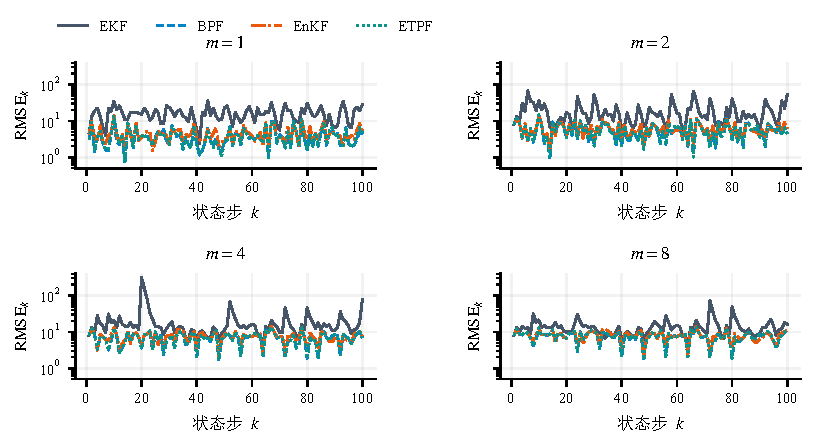
\includegraphics[width=0.84\linewidth]{figs/completed_work/rmse_time.pdf}
\par\vspace{3pt}
{\wuhao 注：取 $N=500$，$\varepsilon=1$，各子图采用相同对数纵轴\par\vspace{2pt}}
\caption{不同观测间隔下的逐时刻跨轨迹 RMSE}
\label{cw:fig:sim-time}
\end{figure}

\begin{figure}[!htb]
\centering
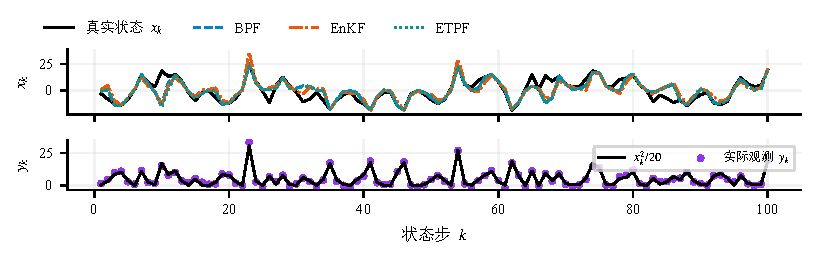
\includegraphics[width=0.84\linewidth]{figs/completed_work/trajectory.pdf}
\par\vspace{3pt}
{\wuhao 注：取 $m=1$，下图对照观测值 $y_k$ 与无噪观测函数 $x_k^2/20$\par\vspace{2pt}}
\caption{首条轨迹的状态与观测序列}
\label{cw:fig:sim-observation}
\end{figure}

\FloatBarrier
\section{粒子数与正则强度及计算开销}

固定 $m=1$ 考察粒子数 $N$、正则参数 $\varepsilon$ 与单步串行耗时（图~\ref{cw:fig:sim-ablation} 与表~\ref{cw:tab:sim-runtime}）。图~\ref{cw:fig:sim-ablation}（a）中，EnKF 在 $N\in\{100,250,500\}$ 下维持在 $5.09$--$5.12$，说明其误差主要受限于线性更新偏差而非样本量。BPF 随 $N$ 单调下降（$4.95\to 4.65$），ETPF（$\varepsilon=1$）在 $N=250$ 时取最低值 $4.57$，$N=500$ 时为 $4.71$：由于算法~\ref{cw:alg:bpf} 与~\ref{cw:alg:etpf} 在重采样前输出相同的加权均值 $X_k^-\bm w_k^+$，两者差异仅通过下一时刻状态传播体现，重心凸组合的轻微方差收缩与 $8$ 条轨迹的抽样波动共同导致了有限样本下的非单调表现。图~\ref{cw:fig:sim-ablation}（b）体现了 $\varepsilon$ 的数值折中（以 $N=500$ 为例）：$\varepsilon=10$ 收敛最快（未收敛率 $1.13\%$），但耦合矩阵趋向秩一乘积而过度收缩方差（RMSE 升至 $4.81$）；$\varepsilon\le 0.1$ 虽更接近精确输运，但 $1000$ 步 Sinkhorn 迭代的未收敛率超过 $78\%$，边际修正后的近似耦合偏离最优解（RMSE 回退至 $4.91$ 以上），故 $\varepsilon=1$ 在平滑偏差与截断误差间较为均衡。

\begin{figure}[!htb]
\centering
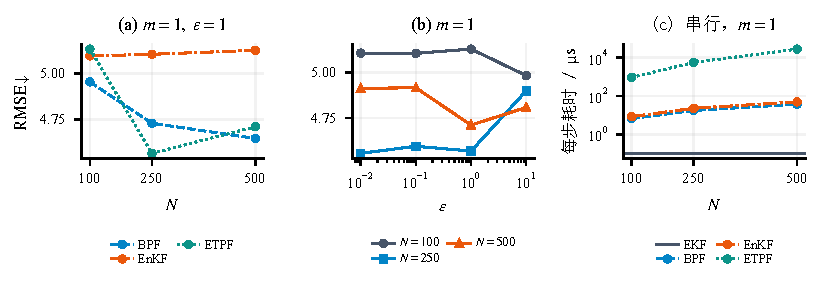
\includegraphics[width=0.88\linewidth]{figs/completed_work/ablation_runtime.pdf}
\par\vspace{3pt}
{\wuhao 注：单因素切片均取 $m=1$\par\vspace{2pt}}
\caption{粒子数与正则强度消融及每步内核耗时}
\label{cw:fig:sim-ablation}
\par\vspace{2pt}
{\wuhao\parbox{\linewidth}{\centering（a）固定 $\varepsilon=1$ 比较 $N$；（b）比较 ETPF 的 $\varepsilon$；（c）固定 $\varepsilon=1$ 的串行单核每步耗时}}
\end{figure}

计算开销上（图~\ref{cw:fig:sim-ablation}（c）与表~\ref{cw:tab:sim-runtime}），当 $N$ 由 $100$ 增至 $500$ 时，BPF（$6.79\to 38.01\,\mu\mathrm{s}$）与 EnKF（$8.50\to 49.68\,\mu\mathrm{s}$）呈 $O(N)$ 增长；ETPF 则由 $0.95\,\mathrm{ms}$ 增至 $28.29\,\mathrm{ms}$（增幅 $29.9$ 倍，$N=500$ 时约为 BPF 的 $744$ 倍），耗时集中于每轮 $O(N^2)$ 的 Sinkhorn 矩阵缩放。图~\ref{cw:fig:sim-density} 的后验密度对比了四类近似的分布形态：$k=11$ 存在符号歧义时，BPF 与 ETPF 均保留双峰且主峰对齐真值，EKF 锁定于错误的负峰，EnKF 则将单峰铺在两峰之间的低密度区；$k=21$ 回归单峰后四者主峰一致，ETPF 方差（$4.41$）略窄于 BPF（$5.08$）。由于该基准的过程噪声较强（方差为 $10$），每步预测扩散足以打散复制粒子，BPF 已能以 $O(N)$ 开销达到相近精度。

\begin{figure}[!htb]
\centering
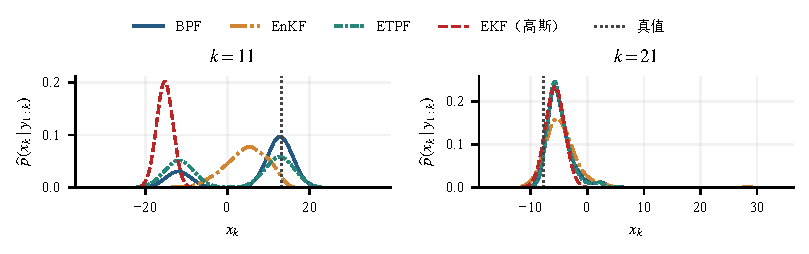
\includegraphics[width=0.88\linewidth]{figs/completed_work/posterior_density.pdf}
\par\vspace{3pt}
{\wuhao 注：取 $m=1$，$N=500$，$\varepsilon=1$\par\vspace{2pt}}
\caption{首条轨迹的后验密度估计对比}
\label{cw:fig:sim-density}
\end{figure}

% 先收束 Gordon 基准图表，避免混入后续 Logistic 实验。
\FloatBarrier
% !TeX root = ../../../main.tex
\section{零过程噪声下粒子贫化与稳健性}\label{cw:sec:sim-logistic}
为剥离过程噪声对粒子多样性的补充并验证定理~\ref{cw:thm:four-errors} 与定理~\ref{cw:thm:bpf-impoverishment}，考察零过程噪声下的确定性混沌 Logistic 映射与平方观测：
\begin{equation}\label{cw:eq:sim-logistic-model}
\begin{aligned}
&X_k=4X_{k-1}(1-X_{k-1}),\quad X_k\in[0,1],\\
&Y_k=h(X_k)+N_{y,k},\quad h(x)=x^2,\quad
X_0\sim U[0,1],\quad N_{y,k}\sim\mathcal N(0,0.1).
\end{aligned}
\end{equation}
取 $N=128$，共 $64$ 条独立路径，每条 $1000$ 步并独立重复运行 $32$ 次（共 $2048$ 次）。BPF 采用每步多项重采样；ETPF 采用一维排序分位数精确最优输运（$O(N\log N)$），不引入熵正则与迭代截断误差。Bayes 参考风险由 $16384$ 格有限体积法计算，不同粒子位置数 $D_k$ 按双精度精确去重统计。

图~\ref{cw:fig:sim-logistic-robustness}（b）验证了定理~\ref{cw:thm:bpf-impoverishment}：BPF 在全部 $2048$ 次运行中均贫化为单点（$D_k=1$），首次单点步数中位数为 $16$（最晚第 $55$ 步）。ETPF 则无一次发生单点贫化，末步平均保留 $69.67$ 个不同位置：一维最优输运中，当高权重粒子质量超过 $1/N$ 时，跨越等质量分界线的目标槽位会对相邻源粒子作凸组合插值，从而在零过程噪声下持续生成内部支撑点。

\begin{table}[!htb]
\centering
\caption{Logistic 模型的四项误差与实测总 MSE}
\label{cw:tab:sim-logistic-errors}
\vspace{0.5em}\wuhao
\sbox0{% !TeX root = ../../../main.tex
\begin{tabular}{lrr}
\toprule[1.5pt]
误差项 & BPF & ETPF \\
\midrule[1pt]
不可约 Bayes 误差 & 0.048755 & 0.048755 \\
算法偏差平方 & 0.075192 & 0.002376 \\
算法随机波动 & 0.123494 & 0.021038 \\
当前重采样扰动 & $4.48\times10^{-6}$ & $5.03\times10^{-31}$ \\
\midrule[1pt]
实测总 MSE & 0.247544 & 0.072128 \\
\bottomrule[1.5pt]
\end{tabular}
}%
\usebox0
\par\vspace{3pt}
\parbox{\wd0}{\wuhao\hspace*{\ccwd}注：表中数值为第 $1$--$1000$ 步平均}
\end{table}

\begin{figure}[!htb]
\centering
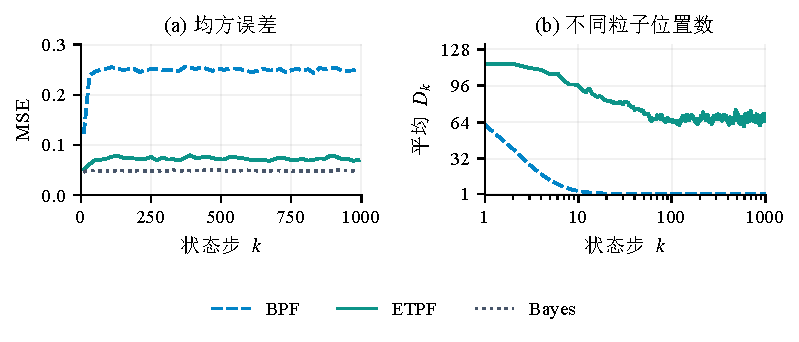
\includegraphics[width=0.88\linewidth]{figs/completed_work/logistic_robustness.pdf}
\par\vspace{3pt}
\caption{Logistic 模型同一批运行的误差与粒子多样性}
\label{cw:fig:sim-logistic-robustness}
\par\vspace{2pt}
{\wuhao\parbox{0.92\linewidth}{\centering（a）每 $20$ 步分段平均的 MSE 与 Bayes 参考风险；（b）重采样后不同位置数的跨运行平均（对数横轴）}}
\end{figure}

表~\ref{cw:tab:sim-logistic-errors} 与图~\ref{cw:fig:sim-logistic-robustness}（a）按式~\eqref{cw:eq:four-errors} 对重采样后均值 $\hat X_k=X_k^+\mathbf1_N/N$ 统计第 $1$--$1000$ 步平均的四项误差（有限样本交叉项仅 $10^{-7}$--$10^{-4}$ 量级）。ETPF 的当前重采样扰动为 $5.03\times 10^{-31}$，数值上为零，验证了质心守恒。值得注意的是，BPF 的当前重采样扰动均值同样很小（$4.48\times 10^{-6}$）：这是因为第 $55$ 步前粒子已全部塌缩为单点，此后重采样当步扰动恒为零，同时似然更新退化为 $w_k^+=1$ 而失去观测修正能力；塌缩后的单点沿混沌映射自由演化至 $\mathrm{Beta}(1/2,1/2)$ 平稳分布（方差 $1/8=0.125$），致使稳态段随机波动升至 $0.125$，总 MSE 接近两独立轨道之差的方差 $0.250$。相比之下，ETPF 将算法偏差平方由 $0.075192$ 降至 $0.002376$，算法随机波动由 $0.123494$ 降至 $0.021038$，总 MSE 降低 $70.9\%$ 至 $0.072128$（其中不可约 Bayes 误差占 $0.048755$），体现了确定性输运对零过程噪声粒子贫化的稳健性。

\FloatBarrier
% !TeX root = ../../../main.tex
\section{高维手写数字序贯识别实验}\label{cw:sec:ml-experiments}

第~\ref{cw:sec:sim-logistic}~节在一维零过程噪声系统上表明，离散最优输运可通过相邻源粒子的分位数凸插值避免单点坍缩。为进一步检验观测空间跃升至高维且潜空间达到十余维时，基于似然权重的离散变换与无权重的连续条件输运映射（第~\ref{cw:sec:ml-transport-theory}~节与第~\ref{cw:sec:ml-updates}~节）各自的表现边界，本节在 MNIST 手写数字数据集\cite{lecun1998gradient}上开展逐窗口含噪序贯识别实验。

\subsection{实验设置与评价指标}

实验采用 MNIST 标准划分中的 $M=60000$ 幅训练图像（像素归一化至 $[0,1]$ 并展平为 $n_D=784$ 维向量）拟合网络与经验先验，取测试集前 $500$ 幅图像开展定量评估。潜空间维数设为 $n_d=16$，压缩算子 $\mathscr T_{\Rightarrow}$、还原算子 $\mathscr T_{\Leftarrow}$ 与类别读出映射 $\ell$ 均采用多层全连接网络实现；在无噪完整测试图像上直接执行压缩与读出（$\ell\circ\mathscr T_{\Rightarrow}$）的测试重构均方误差为 $0.0093$，分类准确率为 $97.8\%$，作为各序贯滤波方法的性能上限参照。序贯观测按式~\eqref{cw:eq:ml-model} 生成：局部窗口边长取 $r=7$，按自左向右、自上而下的无重叠顺序分 $K=16$ 步扫完全图，窗口观测噪声标准差取 $\sigma=0.3$，默认粒子规模为 $N=256$。

实验共对比五种潜空间更新方案：
（1）\textbf{BPF}：每步按式~\eqref{cw:eq:ml-weights} 计算似然权重并执行多项重采样；
（2）\textbf{BPF 加扰动}：在多项重采样后对潜空间粒子叠加强度为 $0.1$ 的各向同性正态扰动，作为缓解零过程噪声粒子贫化的启发式基线；
（3）\textbf{ETPF}：熵正则化强度取当步代价矩阵均值的 $0.005$ 倍，执行 $50$ 轮稳定化交替尺度缩放（Sinkhorn 迭代）；
（4）\textbf{逐步在线 OTPF}：依据文献\cite{aljarrah2024brenier} 的极大极小框架独立复现，每步在线执行 $300$ 轮外层迭代（检验网络每更新 $1$ 次，输运网络更新 $5$ 次），并将 $49$ 维窗口观测投影至前 $4$ 个主特征方向以稳定小样本对抗训练；为确保基线充分调优，ETPF 与逐步 OTPF 的关键超参数均在测试集前 $100$ 幅图像上网格择优固定；
（5）\textbf{静态摊销 OTPF}（算法~\ref{cw:alg:amortized-otpf}）：离线阶段以批量大小 $1024$、内层比例 $5:1$ 训练 $240\,\mathrm{s}$，在线阶段仅执行式~\eqref{cw:eq:ml-amortized-update} 的单次前向映射。

评估采用四项互补指标：（i）式~\eqref{cw:eq:ml-vote} 粒子众数判决的识别准确率；（ii）类别后验平方误差，定义为粒子读出类别经验频率向量与真实类别独热示性向量之差的平方二范数，用于精细衡量后验概率校准程度；（iii）还原均方误差，即等权后验粒子经还原算子解码所得均值图像与真实无噪图像的像素均方误差；（iv）每幅测试图像每个观测步的平均在线推理耗时（批量并行计时）。主实验固定网络参数，以 $3$ 个独立随机种子重复抽样初始先验粒子与观测噪声序列，汇报均值与样本标准差。

\subsection{主要实验结果与机制分析}

\begin{table}[!htb]
\centering
\caption{MNIST 逐窗口序贯数字识别主实验结果}
\label{cw:tab:ml-main}
\vspace{0.5em}\wuhao\setlength{\tabcolsep}{5pt}
\begin{tabular}{lccccc}
\toprule[1.5pt]
 & \multicolumn{2}{c}{识别准确率（\%）$\uparrow$} & 类别后验 & 还原 & 每步在线耗时 \\
方法 & $k=8$ & $k=16$ & 平方误差 $\downarrow$ & 均方误差 $\downarrow$ & （ms）$\downarrow$ \\
\midrule[1pt]
BPF & $49.1\pm3.0$ & $49.2\pm3.1$ & $1.016\pm0.062$ & $0.0762$ & $0.034$ \\
BPF 加扰动 & $51.1\pm1.5$ & $53.9\pm1.7$ & $0.802\pm0.030$ & $0.0527$ & $0.034$ \\
ETPF & $54.3\pm1.4$ & $54.7\pm1.0$ & $0.902\pm0.021$ & $0.0638$ & $0.24$ \\
逐步在线 OTPF & $66.3\pm1.2$ & $81.8\pm1.4$ & $0.286\pm0.023$ & $0.0296$ & $17.2$ \\
静态摊销 OTPF & $\mathbf{92.1}\pm0.9$ & $\mathbf{96.8}\pm0.2$ & $\mathbf{0.045}\pm0.002$ & $\mathbf{0.0124}$ & $\mathbf{0.015}$ \\
\bottomrule[1.5pt]
\end{tabular}
\par\vspace{3pt}
{\wuhao 注：取 $N=256$，$500$ 幅测试图像，$3$ 个随机种子的均值 $\pm$ 标准差；后三列均为全图扫完时刻（$k=16$）的统计值\par}
\end{table}

表~\ref{cw:tab:ml-main} 与图~\ref{cw:fig:ml-curves} 展示了五种方法随观测窗口逐步揭示的定量表现。可以观察到两类截然不同的演化形态：凡依赖似然权重的方法（BPF、BPF 加扰动与 ETPF）均在扫描过半（$k=8$，恰好覆盖图像上半部）前陷入停滞，此后即便下半幅数字笔画完整揭示，识别准确率亦几乎不再增长，末步全部停留在 $49.2\%$--$54.7\%$ 之间。其根源在于 $16$ 维潜空间中的稀疏采样与零过程噪声叠加：对 BPF 而言，前几步局部窗口似然已将不同祖先粒子数由 $256$ 迅速压缩至接近 $1$（图~\ref{cw:fig:ml-curves}（d）离散度归零），一旦锁死于某个仅与上半部笔画相似的错误类别粒子，后续观测便因支撑集单点化而丧失修正能力，直接印证了定理~\ref{cw:thm:bpf-impoverishment}。更值得注意的是，在第~\ref{cw:sec:sim-logistic}~节一维系统中表现优异的 ETPF 在此仅比 BPF 提高 $5.5$ 个百分点：在 $16$ 维空间中，$256$ 个初始粒子高度稀疏，当单步似然权重集中于一两个粒子时，式~\eqref{cw:eq:particle-ot-transform} 的凸组合重心同样收缩至该少数粒子邻域，无法跨越潜空间空白区域生成新的假设模式；人工添加各向同性正态扰动虽维持了表面离散度，但盲目扩散偏离了任务流形方向，同样难以恢复正确类别。

\begin{figure}[!htb]
\centering
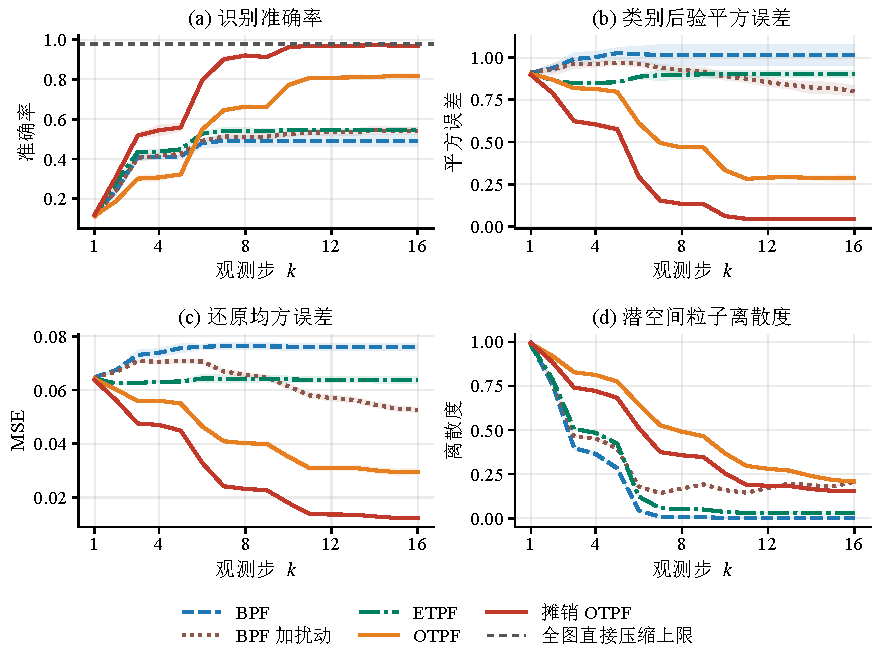
\includegraphics[width=0.94\linewidth]{figs/completed_work/ml_curves.pdf}
\par\vspace{3pt}
{\wuhao 注：实线/虚线为 $3$ 个随机种子的均值，浅色阴影为 $\pm1$ 倍标准差区间；图（a）水平灰虚线表示无噪全图直接压缩读出上限（$97.8\%$）\par\vspace{2pt}}
\caption{五种潜空间滤波方法的各项评价指标随观测步数的演化}
\label{cw:fig:ml-curves}
\end{figure}

\begin{figure}[!htb]
\centering
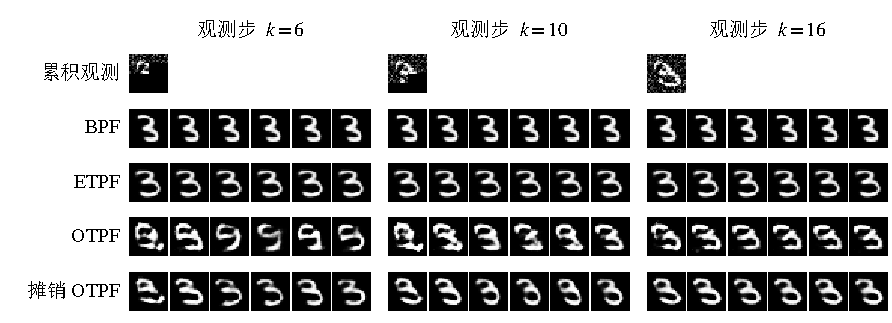
\includegraphics[width=0.96\linewidth]{figs/completed_work/ml_gallery.pdf}
\par\vspace{3pt}
{\wuhao 注：首行为 $k=6,10,16$ 时的含噪累积窗口观测（真实数字为 $3$），其余各行为对应时刻前 $6$ 个等权粒子的还原图像\par\vspace{2pt}}
\caption{单幅测试图像上四类方法的潜空间粒子解码演化对比}
\label{cw:fig:ml-gallery}
\end{figure}

相反，脱离似然权重的两类条件输运映射方法在整个扫描周期内随信息累积持续改善。逐步在线 OTPF 在末步达到 $81.8\%$ 的识别准确率，证明连续神经网络映射可将粒子主动推向任意潜空间区域；但由于每步仅凭 $N=256$ 个合成粒子对开展短期对抗训练，映射近似误差在 $16$ 次递推复合中不断累积，且单步在线训练使每图每步耗时高达 $17.2\,\mathrm{ms}$（约为 BPF 的 $506$ 倍）。静态摊销 OTPF 在半幅观测（$k=8$）时即达到 $92.1\%$，全图观测后达到 $96.8\%$，距无噪全图直接压缩上限（$97.8\%$）仅差 $1.0$ 个百分点，同时类别后验平方误差（$0.045$）与像素还原均方误差（$0.0124$）均显著低于所有对照方法；得益于在线阶段仅需一次前向张量运算，其每步推理耗时仅为 $0.015\,\mathrm{ms}$，比逐步在线 OTPF 快三个数量级。图~\ref{cw:fig:ml-gallery} 直观印证了上述差异：面对真实类别为“$3$”的测试图像，BPF 与 ETPF 在 $k=6$ 时 $6$ 个粒子已完全坍缩为同一固定笔画；逐步 OTPF 保留了多样性但解码轮廓存在局部畸变；静态摊销 OTPF 在早期局部观测存在歧义（$k=6$）时保持“$2$”“$3$”等多种合理笔画假设，随中下部窗口陆续揭示（$k=10,16$）平滑收拢至清晰的真实数字形态。

\subsection{粒子规模与潜空间维数消融}

\begin{table}[!htb]
\centering
\caption{粒子规模 $N$ 对末步识别准确率（$k=16$）的影响}
\label{cw:tab:ml-particles}
\vspace{0.5em}\wuhao
\begin{tabular}{lcccc}
\toprule[1.5pt]
方法 & $N=64$ & $N=256$ & $N=1024$ & $N=4096$ \\
\midrule[1pt]
BPF & $33.2\%$ & $46.6\%$ & $61.0\%$ & $72.0\%$ \\
BPF 加扰动 & $32.6\%$ & $56.2\%$ & $67.2\%$ & $81.4\%$ \\
ETPF & $36.4\%$ & $54.2\%$ & $69.6\%$ & -- \\
静态摊销 OTPF & $\mathbf{96.6\%}$ & $\mathbf{96.8\%}$ & $\mathbf{97.2\%}$ & $\mathbf{97.4\%}$ \\
\bottomrule[1.5pt]
\end{tabular}
\par\vspace{3pt}
{\wuhao 注：单个随机种子评估结果；$N=4096$ 时 ETPF 因 $N\times N$ 耦合矩阵开销过大未予运行\par}
\end{table}

表~\ref{cw:tab:ml-particles} 考察粒子规模 $N\in\{64,256,1024,4096\}$ 对末步准确率的影响（逐步在线 OTPF 因大规模粒子在线训练耗时过高未纳入该组扫描）。三类依赖权重的方法随 $N$ 增大稳步提升，印证了加密初始先验覆盖能够缓解有限支撑漏失；但即便在 $N=4096$ 下，BPF（$72.0\%$）与加扰动基线（$81.4\%$）仍远低于静态摊销 OTPF 在 $N=64$ 时的精度（$96.6\%$）。同时，ETPF 的每步耗时由 $N=256$ 时的 $0.24\,\mathrm{ms}$ 跃升至 $N=1024$ 时的 $7.9\,\mathrm{ms}$（增长逾 $30$ 倍），凸显了 $O(N^2)$ 耦合矩阵缩放在中等粒子规模下的可扩展性瓶颈。静态摊销 OTPF 对粒子规模极不敏感：由于单次映射已直接近似真实条件后验 $\mathbb P_{Z_k\mid Y_{1:k}=y_{1:k}}$，众数分类只需稳健估计十个离散类别的后验概率质量，$N=64$ 个粒子已足以给出低方差判决。

\begin{table}[!htb]
\centering
\caption{潜空间维数 $n_d$ 对重构精度与末步识别准确率的影响}
\label{cw:tab:ml-dim}
\vspace{0.5em}\wuhao
\begin{tabular}{cccccc}
\toprule[1.5pt]
$n_d$ & 测试重构均方误差 $\downarrow$ & 全图直接读出上限 & BPF & ETPF & 静态摊销 OTPF \\
\midrule[1pt]
$8$ & $0.0153$ & $95.5\%$ & $50.4\%$ & $57.6\%$ & $\mathbf{93.6\%}$ \\
$16$ & $0.0093$ & $97.8\%$ & $46.6\%$ & $54.2\%$ & $\mathbf{96.8\%}$ \\
$32$ & $0.0075$ & $98.2\%$ & $47.0\%$ & $55.0\%$ & $\mathbf{96.2\%}$ \\
\bottomrule[1.5pt]
\end{tabular}
\par\vspace{3pt}
{\wuhao 注：取 $N=256$，$k=16$，单个随机种子；$n_d=8,32$ 下摊销网络离线训练预算为 $150\,\mathrm{s}$，$n_d=16$ 下为 $240\,\mathrm{s}$\par}
\end{table}

表~\ref{cw:tab:ml-dim} 进一步考察潜空间维数 $n_d\in\{8,16,32\}$ 的折中效应。随着 $n_d$ 增加，还原流形的表达能力增强，测试重构均方误差单调下降（$0.0153\to0.0075$），全图直接读出上限相应升至 $98.2\%$。与之相对，BPF 与 ETPF 在 $n_d=8$ 时反而略高于 $n_d=16,32$，反映了重要性采样随潜维数升高而加剧的权重退化趋势。静态摊销 OTPF 在三个维数下均稳定逼近各自的全图读出上限；$n_d=32$ 略低于 $n_d=16$（$96.2\%$ 对 $96.8\%$）主要源于补充消融采用了较短的固定离线训练时长（$150\,\mathrm{s}$ 对 $240\,\mathrm{s}$）且高维输运网络收敛略慢。总计计算成本方面，在表~\ref{cw:tab:sim-environment} 所示单张 GPU 环境下，完成主实验全部三个网络的离线训练及五种方法的在线评估共耗时 $426\,\mathrm{s}$（其中摊销映射离线训练占 $240\,\mathrm{s}$，逐步在线 OTPF 评估占 $152\,\mathrm{s}$），包含多种子重复与两项消融在内的完整实验流程总计耗时 $1118\,\mathrm{s}$。


\FloatBarrier
\section{本章小结}

本章在三类具有不同难点特征的任务上检验了前述理论与算法的实际表现。两组一维数值实验首先划清了离散耦合输运的适用边界：在过程噪声较强的 Gordon 模型中，状态转移自身的随机扩散已经足够替粒子集补充多样性，此时开销更低的自举粒子滤波（BPF）就能拿到与集合输运（ETPF）相当的精度，不必盲目付出 $O(N^2)$ 的耦合求解代价；但一旦进入零过程噪声的混沌 Logistic 系统，BPF 在全部实验中均迅速退化为单个点并彻底失去观测修正能力，而精确分位数 ETPF 依靠无复制的位置变换稳住了样本多样性，显著压低了跟踪误差。

在 $784$ 维含噪手写数字逐窗口识别实验中，各种机制的差异进一步拉开。即使已经把观测压缩到了 $16$ 维潜空间，依赖似然权重的 BPF 与 ETPF 仍在最初几步就陷入少数粒子垄断权重的局面，后续窗口的观测信息难以扭转早期判断；逐步在线训练的条件输运映射摆脱了权重限制，识别率明显回升，但受限于有限粒子规模、跨步复合误差以及每步在线训练的时间开销；相比之下，静态摊销条件输运滤波利用离线学到的全局映射每步直接从初始粒子一步推向当前后验，不仅在识别准确率上逼近全图直接读出的上限，还将每步在线耗时压缩到了亚毫秒量级，验证了流形降维与一步摊销输运相结合的有效性。

\backmatter
% !TeX root = ../main.tex
\begin{conclusions}
围绕传统粒子滤波在弱过程噪声下易塌缩为单点、在高维观测下似然权重失效这两类问题，本文结合最优输运与神经网络流形表示开展了理论分析与算法设计，主要结论如下：
\begin{enumerate}[label=(\arabic*),leftmargin=0pt,labelindent=2\ccwd,itemindent=*,labelsep=0.4em,nosep]
  \item 在低维离散重采样层面，建立了粒子重采样更新（涵盖 BPF 与 ETPF）的四项均方误差正交分解，并证明零过程噪声与确定性演化下自举粒子滤波（BPF）的不同粒子位置数期望按指数速率衰减至 $1$；仿真表明，强过程噪声下 BPF 即可低开销维持精度，而零过程噪声混沌系统中 BPF 全部塌缩为单点，ETPF 则完全避免了单点退化并显著降低估计误差。
  \item 在高维观测降维层面，提出了经验模内积下的压缩与还原流形拟合方法，给出平直线性子空间投影的伴随闭式解与谱截断性质，并推广至神经网络参数化的低维子流形，拟合高维观测对象流形以提取紧凑潜坐标并导出数据驱动的潜空间先验。
  \item 在潜空间后验更新层面，引入无需计算似然权重的条件输运映射对抗学习，利用潜状态静止时滤波后验的一步累积性质，提出离线统一训练、在线单次前向推理的静态摊销条件输运滤波算法；在含噪手写数字逐窗口识别实验中，传统加权滤波因权重集中而准确率偏低，逐步在线训练网络虽能提升精度但单步耗时较长，所提静态摊销方法同时实现了接近全图上限的识别准确率与亚毫秒级的单步推理速度。
\end{enumerate}

本文研究仍存在一定局限，后续工作可从以下方面继续推进：
\begin{enumerate}[label=(\arabic*),leftmargin=0pt,labelindent=2\ccwd,itemindent=*,labelsep=0.4em,nosep]
  \item 静态摊销方法的一步更新建立在潜状态不随时间变化的假设之上；面向状态随时间演化的动态系统，后续需引入循环网络或集合编码器汇总历史观测以构造时变条件输运映射。
  \item 离线摊销训练利用了训练集的成对样本，与仅在线访问有限先验粒子的传统加权滤波在已知信息量上并不对等，少样本或测试分布偏移条件下的映射泛化性能仍有待探索。
  \item 高维图像实验缺乏解析真值后验，目前主要借助分类误差与像素还原误差作间接评估，且在线对抗输运基线受限于固定训练步数预算；未来可结合可求解析后验的中高维基准及更大规模的重复实验作进一步检验。
\end{enumerate}
\end{conclusions}

% !TeX root = ../main.tex
\makeatletter
\ifhit@openright\cleardoublepage\else\clearpage\fi
\hit@appendix@chapter*{人工智能使用声明}[AI Use Statement]
\makeatother

根据相关学术规范政策，本文对研究与撰写过程中生成式人工智能（AI）工具的使用情况作如下透明披露：
\begin{enumerate}[label=(\arabic*),leftmargin=0pt,labelindent=2\ccwd,itemindent=*,labelsep=0.4em,nosep]
  \item 文献综述部分的文献检索与前期调研较大幅度使用了 AI 工具辅助，作者负责最终引用文献的筛选、原始出处的溯源以及正文叙述内容的逐项核对。
  \item 文中大部分数学推导的展开细节由作者与 AI 工具协力完成，作者主导问题建模、符号体系设计、可读性校验与理论体系化归纳；对于部分核心定理与命题，作者进一步使用交互式定理证明器 Lean 4 指导 AI 完成了形式化证明核验，以确保推导与证明严格无误。
  \item 仿真与视觉实验的实现代码（除直接引用相关文献的既有开源实现外）由 AI 工具负责编写，全部代码与复现脚本开源托管于 GitHub 仓库（\href{https://github.com/ShouxinZhang/filter-theory-study}{\texttt{https://github.com/ShouxinZhang/filter-theory-study}}）；作者负责依据数学原理设计数值与性质核验模块，在各项核验指标未出现明确异常时予以采纳。
  \item 本文主体内容整合自作者日常研究积累的若干专题笔记；在相关笔记的创作与整理过程中，AI 工具高度参与了协同撰写，作者本人负责全部内容的统合梳理与逐字校对。
\end{enumerate}

除上述辅助环节外，作者对本论文的全部研究结论、文字表述、数学论断与实验结果的真实性及准确性承担完整学术责任。

\bibliography{references/startpaper,references/completed_work}
\begin{appendix}
  % !TeX root = ../main.tex
\chapter{Bayes 滤波引理与更新公式证明}[Proofs for Bayesian Filtering]\label{cw:app:appendix}
% 新证明单独维护，保持附录主干简洁。
% !TeX root = ../../../main.tex
\section{无记忆性引理的离散情形证明}\label{cw:app:markov-proof}

\begin{proof}[引理~\ref{cw:lem:markov} 的证明（离散情形）]
沿用引理~\ref{cw:lem:markov} 的模型与独立性条件，设 $X_0$ 和各噪声取有限或可数个值，$p$ 表示相对于计数测度的概率质量函数。
以下仅考虑概率为正的条件取值，求和遍历相应噪声的所有可能取值。

由递推关系，$(X_{0:k-1},Y_{1:k-1})$ 是 $(X_0,N_{x,1:k-1},N_{y,1:k-1})$ 的函数，因此与 $N_{x,k}$ 独立。
固定历史取值后，$X_{k-1}=x_{k-1}$，先按噪声取值分解，再依次使用 $X_k=f(X_{k-1},N_{x,k})$ 与噪声独立性：
\begin{equation*}
\begin{aligned}
&p_{X_k\mid X_{0:k-1},Y_{1:k-1}}(x_k\mid x_{0:k-1},y_{1:k-1})\\
= &\sum_n p_{(X_k,N_{x,k})\mid X_{0:k-1},Y_{1:k-1}}(x_k,n\mid x_{0:k-1},y_{1:k-1})\\
= &\sum_n\mathbb I_{\{f(x_{k-1},n)=x_k\}}p_{N_{x,k}\mid X_{0:k-1},Y_{1:k-1}}(n\mid x_{0:k-1},y_{1:k-1})\\
= &\sum_n\mathbb I_{\{f(x_{k-1},n)=x_k\}}p_{N_{x,k}}(n)\\
= &p_{X_k\mid X_{k-1}}(x_k\mid x_{k-1}).
\end{aligned}
\end{equation*}
最后一步同样利用 $N_{x,k}$ 与 $X_{k-1}$ 独立，故只给定 $X_{k-1}$ 时得到相同的求和式。

同理，$(X_{0:k},Y_{1:k-1})$ 是 $(X_0,N_{x,1:k},N_{y,1:k-1})$ 的函数，因此与 $N_{y,k}$ 独立。由 $Y_k=h(X_k,N_{y,k})$ 得
\begin{equation*}
\begin{aligned}
&p_{Y_k\mid X_{0:k},Y_{1:k-1}}(y_k\mid x_{0:k},y_{1:k-1})\\
= &\sum_n\mathbb I_{\{h(x_k,n)=y_k\}}p_{N_{y,k}}(n)\\
= &p_{Y_k\mid X_k}(y_k\mid x_k).
\end{aligned}
\end{equation*}
这里最后一步利用 $N_{y,k}$ 与 $X_k$ 独立。$k=1$ 时将历史观测视为空，即得引理的两个等式。

一般情形对任意可测集合写条件概率，将上述求和替换为对噪声分布的积分，即得相同的条件分布等式；在正文的密度存在假设下，进一步得到几乎处处成立的密度等式。
\end{proof}


\section{Bayes 更新公式的证明}\label{cw:app:proofs}

\begin{theorem}[Bayes 更新公式]\label{cw:thm:bayes}

在本文约定与模型条件下，对 $k\geq1$，给定历史观测 $y_{1:k-1}$ 并收到当前观测 $y_k$ 后，状态后验密度满足
\begin{equation}\label{cw:eq:15}
\begin{aligned}
&p_{X_k\mid Y_{1:k}}(x_k\mid y_{1:k})\\
= &\frac{p_{Y_k\mid X_k}(y_k\mid x_k)p_{X_k\mid Y_{1:k-1}}(x_k\mid y_{1:k-1})}
{\displaystyle\int_{\mathcal{S}_X}p_{Y_k\mid X_k}(y_k\mid x)p_{X_k\mid Y_{1:k-1}}(x\mid y_{1:k-1})\,\mathrm{d}v_X(x)}.
\end{aligned}
\end{equation}

\end{theorem}

\begin{proof}
经典结论参见文献\cite{sarkka2013bayesian,cappe2005inference}；为完整起见，下面给出自行推导的证明。

先固定历史观测 $y_{1:k-1}$。收到 $y_k$ 后，要求的是在这些历史观测的基础上，再给定 $Y_k=y_k$ 时的状态密度。按条件密度公式，将条件联合密度除以新观测的条件边缘密度：
\begin{equation}\label{cw:eq:16}
\begin{aligned}
&p_{X_k\mid Y_{1:k}}(x_k\mid y_{1:k})\\
= &\frac{p_{(X_k,Y_k)\mid Y_{1:k-1}}(x_k,y_k\mid y_{1:k-1})}
{p_{Y_k\mid Y_{1:k-1}}(y_k\mid y_{1:k-1})}.
\end{aligned}
\end{equation}

对分子使用密度的乘法公式，按“先取状态，再给定状态取观测”的顺序分解。两个因子都保留历史观测条件，其中状态因子正是预测步骤已求得的密度：
\begin{equation}\label{cw:eq:17}
\begin{aligned}
&p_{(X_k,Y_k)\mid Y_{1:k-1}}(x_k,y_k\mid y_{1:k-1})\\
= &p_{Y_k\mid X_k,Y_{1:k-1}}(y_k\mid x_k,y_{1:k-1})
p_{X_k\mid Y_{1:k-1}}(x_k\mid y_{1:k-1}).
\end{aligned}
\end{equation}
将这一分解代入上一式，就是以历史观测为条件的 Bayes 公式。

接着应用无记忆性引理中的观测条件独立性。给定当前状态 $X_k$ 后，历史观测不再影响 $Y_k$ 的条件分布，因此观测因子可以直接使用模型给出的似然：
\begin{equation}\label{cw:eq:18}
p_{Y_k\mid X_k,Y_{1:k-1}}(y_k\mid x_k,y_{1:k-1})
=p_{Y_k\mid X_k}(y_k\mid x_k).
\end{equation}
这里仅消去了观测因子中的历史条件，预测密度仍依赖历史观测。

分母由条件联合密度对状态变量积分得到，这是条件全概率公式。再代入上面的乘法分解与条件独立关系，就将观测的预测密度写成似然关于状态预测分布的平均：
\begin{equation}\label{cw:eq:19}
\begin{aligned}
&p_{Y_k\mid Y_{1:k-1}}(y_k\mid y_{1:k-1})\\
= &\int_{\mathcal{S}_X}p_{(X_k,Y_k)\mid Y_{1:k-1}}(x,y_k\mid y_{1:k-1})\,\mathrm{d}v_X(x)\\
= &\int_{\mathcal{S}_X}p_{Y_k\mid X_k}(y_k\mid x)
p_{X_k\mid Y_{1:k-1}}(x\mid y_{1:k-1})\,\mathrm{d}v_X(x).
\end{aligned}
\end{equation}
其中 $x$ 是积分变量，覆盖整个状态空间。按前述条件，这个分母有限且严格为正，可以用于归一化。

最后，将得到的分子与分母代回最初的条件密度公式，即得定理中的更新式。分母是似然加权后预测密度的总积分，因此相除后得到积分为 $1$ 的后验密度。
\end{proof}

  % !TeX root = ../main.tex
\chapter{离散 Monge 映射的存在条件}[Existence Condition for Discrete Monge Maps]\label{cw:app:monge}

\textbf{原子质量守恒：}设 $x_1,\dots,x_m$ 各自互异，$y_1,\dots,y_n$ 各自互异，$a_i,b_j>0$。若 $T_*\mathbb P_X=\mathbb P_Y$，则
\begin{equation}\label{cw:eq:monge-atom-mass}
\begin{aligned}
b_j&=\mathbb E_{Y\sim\mathbb P_Y}[\mathbb I_{\{y_j\}}(Y)]
=\mathbb E_{X\sim\mathbb P_X}[\mathbb I_{\{y_j\}}(T(X))]\\
&=\int_{\mathcal S_X}\mathbb I_{\{y_j\}}(T(x))\,
\mathrm d\!\left(\sum_{i=1}^m a_i\delta_{x_i}\right)(x)
=\sum_{\{i:\,T(x_i)=y_j\}}a_i.
\end{aligned}
\end{equation}
每个正质量源点必然映入目标支撑，因为
\begin{equation}\label{cw:eq:monge-support}
\mathbb P_Y(\{T(x_i)\})
=\mathbb P_X(T^{-1}(\{T(x_i)\}))\ge a_i>0.
\end{equation}
因此其条件概率矩阵为逐行单点选择，联合概率矩阵则带有源权重：
\begin{equation}\label{cw:eq:monge-conditional}
\begin{aligned}
&P_{Y\mid X;i,j}=\mathbb I_{\{y_j\}}(T(x_i))\in\{0,1\},\qquad
\sum_{j=1}^n P_{Y\mid X;i,j}
=\delta_{T(x_i)}\!\left(\bigcup_{j=1}^n\{y_j\}\right)=1,\\
&\bm P_{Y\mid X}\mathbf1_n=\mathbf1_m,\qquad
\bm P_{Y\mid X}^{\mathrm T}\bm a=\bm b,\qquad
\bm\Pi=\operatorname{diag}(\bm a)\bm P_{Y\mid X}.
\end{aligned}
\end{equation}
同一质量关系也可以完全用推前与拉回对偶表达：
\begin{equation}\label{cw:eq:monge-duality}
\begin{aligned}
b_j&=\langle\mathbb I_{\{y_j\}},\mathbb P_Y\rangle_{\mathcal S_Y}
=\langle\mathbb I_{\{y_j\}},T_*\mathbb P_X\rangle_{\mathcal S_Y}
=\langle T^*\mathbb I_{\{y_j\}},\mathbb P_X\rangle_{\mathcal S_X}\\
&=\left\langle T^*\mathbb I_{\{y_j\}},
\delta_{x_{1..m}}\bm a\right\rangle_{\mathcal S_X}
=\sum_{i=1}^m a_iP_{Y\mid X;i,j}.
\end{aligned}
\end{equation}

% 保留定理陈述的最小空间，证明可自然跨页，不预留半页。
\Needspace{5\baselineskip}
\begin{theorem}[均匀离散分布的整除条件]\label{cw:thm:monge-divisibility}
设源、目标分布分别均匀分布于 $m$ 个与 $n$ 个互异支撑点。存在可测映射 $T$ 满足 $T_*\mathbb P_X=\mathbb P_Y$，当且仅当 $n\mid m$。
\end{theorem}
\begin{proof}
必要性：由式~\eqref{cw:eq:monge-atom-mass}，每个目标点的原像必须含有 $m/n$ 个源点：
\begin{equation}\label{cw:eq:monge-divisibility}
\frac1n=\frac1m\#\{i:T(x_i)=y_j\}
\quad\Longrightarrow\quad\frac mn\in\mathbb N.
\end{equation}
充分性：若 $m=nq$，将每 $q$ 个源点分配给一个目标点。用矩阵分块直积写为
\begin{equation}\label{cw:eq:monge-construction}
\begin{aligned}
&\bm P_{Y\mid X}=\bm I_n\otimes_k\mathbf1_q\in\{0,1\}^{m\times n},
\qquad\bm\Pi=\frac1m\bm P_{Y\mid X},\\
&\bm P_{Y\mid X}\mathbf1_n
=(\bm I_n\otimes_k\mathbf1_q)(\mathbf1_n\otimes_k1)
=\mathbf1_n\otimes_k\mathbf1_q=\mathbf1_m,\\
&\bm P_{Y\mid X}^{\mathrm T}\frac{\mathbf1_m}{m}
=\frac{(\bm I_n\otimes_k\mathbf1_q^{\mathrm T})(\mathbf1_n\otimes_k\mathbf1_q)}m
=\frac q m\mathbf1_n=\frac1n\mathbf1_n.
\end{aligned}
\end{equation}
以矩阵每行的唯一非零元素确定 $T(x_i)$，并在有限源支撑之外任取常值延拓，即得到所需可测映射。
\end{proof}

  % !TeX root = ../main.tex
\chapter{线性流形正交投影与谱截断证明}[Proofs of Orthogonal Projection and Spectral Truncation]\label{cw:app:manifold}

本附录给出命题~\ref{cw:prop:linear-manifold} 中两项结论的完整推导。

\section{正交投影与最优压缩算子的伴随表达式}

设有限维完备内积空间 $\mathcal S_Z$（$\dim\mathcal S_Z=n_d$）到完备内积空间 $\mathcal S_X$ 的单射线性算子为 $\mathscr T_{\Leftarrow}:\mathcal S_Z\to\mathcal S_X$，记像子空间为 $W:=\operatorname{im}(\mathscr T_{\Leftarrow})<\mathcal S_X$。内积伴随算子 $\mathscr T_{\Leftarrow}^{\star}:\mathcal S_X\to\mathcal S_Z$ 由下式唯一确定：
\begin{equation}\label{cw:eq:app-adjoint-def}
\langle\mathscr T_{\Leftarrow}v\mid x\rangle_{\mathcal S_X}
=\langle v\mid\mathscr T_{\Leftarrow}^{\star}x\rangle_{\mathcal S_Z},\qquad
\forall v\in\mathcal S_Z,\ x\in\mathcal S_X.
\end{equation}
对任意 $x\in\mathcal S_X$，因 $\mathscr P_W x\in\operatorname{im}(\mathscr T_{\Leftarrow})$ 且 $\mathscr T_{\Leftarrow}$ 单射，存在唯一 $u\in\mathcal S_Z$ 使得 $\mathscr P_W x=\mathscr T_{\Leftarrow}u$。由正交分解定理，余投影向量满足 $x-\mathscr T_{\Leftarrow}u\perp W$，即对任意 $v\in\mathcal S_Z$ 有
\begin{equation}\label{cw:eq:app-normal-eq}
0=\bigl\langle\mathscr T_{\Leftarrow}v\bigm|x-\mathscr T_{\Leftarrow}u\bigr\rangle_{\mathcal S_X}
=\bigl\langle v\bigm|\mathscr T_{\Leftarrow}^{\star}(x-\mathscr T_{\Leftarrow}u)\bigr\rangle_{\mathcal S_Z}
\iff\mathscr T_{\Leftarrow}^{\star}\mathscr T_{\Leftarrow}u=\mathscr T_{\Leftarrow}^{\star}x.
\end{equation}
对任意非零 $v\in\mathcal S_Z$，由 $\mathscr T_{\Leftarrow}$ 的单射性知
\begin{equation}
\langle v\mid\mathscr T_{\Leftarrow}^{\star}\mathscr T_{\Leftarrow}v\rangle_{\mathcal S_Z}
=\|\mathscr T_{\Leftarrow}v\|_{\mathcal S_X}^2>0,
\end{equation}
故自伴算子 $\mathscr T_{\Leftarrow}^{\star}\mathscr T_{\Leftarrow}:\mathcal S_Z\to\mathcal S_Z$ 严格正定从而可逆。在式~\eqref{cw:eq:app-normal-eq} 两端左乘 $(\mathscr T_{\Leftarrow}^{\star}\mathscr T_{\Leftarrow})^{-1}$ 解出 $u=(\mathscr T_{\Leftarrow}^{\star}\mathscr T_{\Leftarrow})^{-1}\mathscr T_{\Leftarrow}^{\star}x$，代回 $\mathscr P_W x=\mathscr T_{\Leftarrow}u$ 并结合单射性，即得一般伴随形式下的正交投影与最优压缩算子：
\begin{equation}\label{cw:eq:app-adjoint-proj}
\mathscr P_W=\mathscr T_{\Leftarrow}\bigl(\mathscr T_{\Leftarrow}^{\star}\mathscr T_{\Leftarrow}\bigr)^{-1}\mathscr T_{\Leftarrow}^{\star},\qquad
\mathscr T_{\Leftarrow}\mathscr T_{\Rightarrow}=\mathscr P_W
\iff\mathscr T_{\Rightarrow}^{\optstar}=\bigl(\mathscr T_{\Leftarrow}^{\star}\mathscr T_{\Leftarrow}\bigr)^{-1}\mathscr T_{\Leftarrow}^{\star}.
\end{equation}
当 $\mathcal S_X=\mathbb R^{n_D},\mathcal S_Z=\mathbb R^{n_d}$ 均赋予标准实内积时，$\mathscr T_{\Leftarrow}^{\star}$ 在标准基下的表示矩阵即为转置矩阵 $\bm T_{\Leftarrow}^{\mathrm T}$（复标准内积下为共轭转置 $\bm T_{\Leftarrow}^{\mathrm H}$），从而给出 $\bm T_{\Rightarrow}^{\optstar}=(\bm T_{\Leftarrow}^{\mathrm T}\bm T_{\Leftarrow})^{-1}\bm T_{\Leftarrow}^{\mathrm T}$，此时式~\eqref{cw:eq:manifold-orth-decomp} 右端第二项恒等于零。

\section{最优平直真子空间的谱截断推导}

由 $\bm P_W^{\perp}=\bm I_{n_D}-\bm P_W$ 可知，在子空间维数约束 $\dim W=n_d$ 下极小化余投影重构误差 $\operatorname{tr}\bigl(\bm P_W^{\perp}\langle x_{1..M}\mid x_{1..M}\rangle_{\hat{\mathbb P}_M}\bigr)$，等价于极大化正交投影捕获能量 $\operatorname{tr}\bigl(\bm P_W\langle x_{1..M}\mid x_{1..M}\rangle_{\hat{\mathbb P}_M}\bigr)$。

因经验二阶矩矩阵 $\langle x_{1..M}\mid x_{1..M}\rangle_{\hat{\mathbb P}_M}=\frac1M x_{1..M}x_{1..M}^{\mathrm T}\in\mathbb R^{n_D\times n_D}$ 实对称半正定，存在规范正交特征向量族 $u_{1..n_D}$ 与非负特征值 $\lambda_1\ge\dots\ge\lambda_{n_D}\ge0$，使其正交谱分解写为
\begin{equation}\label{cw:eq:app-spectral-decomp}
\langle x_{1..M}\mid x_{1..M}\rangle_{\hat{\mathbb P}_M}
=\sum_{j=1}^{n_D}\lambda_j\bm P_{u_j},\qquad
\bm P_{u_j}:=u_ju_j^{\mathrm T}.
\end{equation}
对每个 $j\in\{1,\dots,n_D\}$，利用正交投影矩阵的对称性与幂等性（$\bm P_W^{\mathrm T}=\bm P_W=\bm P_W^2$）有
\begin{equation}
\operatorname{tr}(\bm P_W\bm P_{u_j})
=\operatorname{tr}(\bm P_W u_ju_j^{\mathrm T})
=u_j^{\mathrm T}\bm P_W u_j
=\|\bm P_W u_j\|^2\in[0,1].
\end{equation}
又由正交规范基的完备性 $\sum_{j=1}^{n_D}\bm P_{u_j}=\bm I_{n_D}$ 及子空间维数 $\dim W=n_d$，各特征方向上的投影范数平方和满足守恒关系
\begin{equation}
\sum_{j=1}^{n_D}\|\bm P_W u_j\|^2
=\operatorname{tr}\!\left(\bm P_W\sum_{j=1}^{n_D}\bm P_{u_j}\right)
=\operatorname{tr}(\bm P_W)=n_d.
\end{equation}
将谱分解式~\eqref{cw:eq:app-spectral-decomp} 代入目标迹，并以第 $n_d$ 个特征值 $\lambda_{n_d}$ 为分界拆项放缩：
\begin{equation}\label{cw:eq:app-spectral-bound}
\begin{aligned}
\operatorname{tr}\bigl(\bm P_W\langle x_{1..M}\mid x_{1..M}\rangle_{\hat{\mathbb P}_M}\bigr)
&=\sum_{j=1}^{n_D}\lambda_j\|\bm P_W u_j\|^2\\
&=\lambda_{n_d}\sum_{j=1}^{n_D}\|\bm P_W u_j\|^2+\sum_{j=1}^{n_D}(\lambda_j-\lambda_{n_d})\|\bm P_W u_j\|^2\\
&\le n_d\lambda_{n_d}+\sum_{j=1}^{n_d}(\lambda_j-\lambda_{n_d})
=\sum_{j=1}^{n_d}\lambda_j,
\end{aligned}
\end{equation}
其中不等号利用了对 $j\le n_d$ 有 $\lambda_j-\lambda_{n_d}\ge0$ 且 $\|\bm P_W u_j\|^2\le1$，对 $j>n_d$ 有 $\lambda_j-\lambda_{n_d}\le0$ 且 $\|\bm P_W u_j\|^2\ge0$。当取 $W^{\optstar}=\operatorname{span}\{u_1,\dots,u_{n_d}\}$（即 $\bm P_{W^{\optstar}}=\sum_{j=1}^{n_d}\bm P_{u_j}$）时，对 $j\le n_d$ 有 $\|\bm P_{W^{\optstar}}u_j\|^2=1$，对 $j>n_d$ 有 $\|\bm P_{W^{\optstar}}u_j\|^2=0$，式~\eqref{cw:eq:app-spectral-bound} 取得等号。故最小余投影重构误差为
\begin{equation}
\operatorname{tr}\bigl(\langle x_{1..M}\mid x_{1..M}\rangle_{\hat{\mathbb P}_M}\bigr)-\sum_{j=1}^{n_d}\lambda_j
=\sum_{j=n_d+1}^{n_D}\lambda_j,
\end{equation}
且当谱间隙满足 $\lambda_{n_d}>\lambda_{n_d+1}$ 时，等号成立当且仅当 $\bm P_W u_j=u_j$（$j\le n_d$）及 $\bm P_W u_j=\bm 0$（$j>n_d$），最优子空间 $W^{\optstar}$ 唯一。

\end{appendix}
% !TeX root = ../main.tex
\begin{publication}
\noindent\textbf{（一）发表的学术论文}

无。

\vspace{0.5\baselineskip}
\noindent\textbf{（二）其他成果}
\begin{publist}
\item 开发了面向数学研究（AI4Math）的若干智能体技能（Agent Skills），开源托管于 GitHub：\url{https://github.com/ShouxinZhang/filter-theory-study}。
\end{publist}
\end{publication}

\authorization
% !TeX root = ../main.tex
\begin{acknowledgements}
严质彬教授对本文的滤波相关数学理论作出了严格而精确的指导，并对本文若干初期灵感进行了敏捷评估。
\end{acknowledgements}

\end{document}
